\usepackage[notref,notcite]{showkeys}
%\usepackage{hyperref}
\usepackage{tikz}
\usetikzlibrary{svg.path}
\excludecomment{solution}
\tikzset{velox/.style={color=black,draw,fill=red,thick,%
    shape=diamond,aspect=.4,
    inner sep=1.3pt,transform shape}}
\tikzset{veloy/.style={color=black,draw,fill=red,thick,%
    shape=diamond,aspect=2.5,
    inner sep=1.3pt,transform shape}}
\tikzset{veloxy/.style={color=black,draw,fill=red,thick,%
    shape=star,star points=4,star point ratio=2.2,
    inner sep=1.3pt,transform shape}}
\tikzset{pressure/.style={color=black,draw,fill=cyan,thick,%
    shape=circle,inner sep=2pt,transform shape}}
\tikzset{velo/.style={transform shape,double=red,arrows={-Stealth[open,fill=red]}}}

%% Macros for drawing degrees of freedom for different shapes/elements.
%% Arguments are always:
%%   #1: Starting point
%%   #2: End point
%%   #3: polynomial degree
%%   #4: node settings

\tikzset{pics/edgenormal/.style args={#1/#2/#3/#4}{%
    code={%
      \draw #1 -- #2
      node foreach \x [evaluate=\x as \xval] in {1,...,#3} [#4,sloped,pos=\xval/(#3+1)] {};
      }
}}


%% Macros for drawing degrees of freedom for different shapes/elements.
%% Arguments are always:
%%   #1: polynomial degree
%%   #2: node settings

\tikzset{pics/tripile/.style args={#1/#2}{%
    code={%
      \coordinate (top) at (0,#1);
      \foreach \i in{0,...,#1}
      \foreach \j in{0,...,\i}
      {
        \tikzmath{
          \y = .3*(2/3*#1-\i)*cos(30);
          \x = .3*(\i/2-\j);
        }
        \node[#2] at (\x,\y) {};
      }
    }
}}

\tikzset{pics/tensor/.style args={#1/#2/#3}{%
    code={%
      \coordinate (top) at (0,#1);
      \foreach \i in{0,...,#1}
      \foreach \j in{0,...,#2}
      {
        \tikzmath{
          \y = 2*(\i+1)/(#1+2);
          \x = 2*(\j+1)/(#2+2);
        }
        \node[#3] at (\x,\y) {};
      }
    }
}}

\tikzset{pics/pfem/.style args={#1/#2}{%
    code={%
      \tikzmath{ \ytop=2*cos(30); }
      \coordinate (top) at (0,\ytop);

      \foreach \i in{0,...,#1}
      \foreach \j in{0,...,\i}
      {
        \tikzmath{
          \y = \ytop-\ytop*\i/#1;
          \x = 2*(\i/2-\j)/#1+1;
        }
        \node[#2] at (\x,\y) {};
      }
    }
}}

\tikzset{pics/qfem/.style args={#1/#2}{%
    code={%
      \foreach \i in{0,...,#1}
      \foreach \j in{0,...,#1}
      {
        \tikzmath{
          \y = 2-2*\i/#1;
          \x = 2-2*\j/#1;
        }
        \node[#2] at (\x,\y) {};
      }
    }
}}

%%% Local Variables:
%%% mode: latex
%%% TeX-master: "all"
%%% End:


\def\constref#1{C_{\text{\ref{#1}}}}
\title{Finite Elements}
\author{Guido Kanschat}
\date{\today}

\begin{document}
\maketitle

\chapter{Elliptic PDE and Their Weak Formulation}
\section{Elliptic boundary value problems}
\subsection{Linear second order PDE}

\begin{Notation}{coordinates}
  Dimension of ``physical space'' will be denoted by $d$.  We denote
  coordinates in $\R^d$ as
  \begin{gather*}
    \vx = (x_1,\dots,x_d)^T  .
  \end{gather*}
  In the special cases $d=2,3$ we also write
  \begin{gather*}
  \vx =
  \begin{pmatrix}
    x\\y
  \end{pmatrix},
  \qquad\qquad
  \vx = \begin{pmatrix}
    x\\y\\z
  \end{pmatrix},
  \end{gather*}
  respectively.
  The Euclidean norm on $\R^d$ is denoted as
  \begin{gather*}
     \abs{\vx} = \sqrt{\sum_{i=1}^d x_i^2}.
  \end{gather*}
\end{Notation}

\begin{Notation}{partial-derivative}
  Partial derivatives of a function $u\in C^1(\R^d)$ are denoted by
  \begin{gather*}
    \frac{\d u(\vx)}{\d x_i} = \tfrac{\d}{\d x_i} u(\vx)
    = \d_{x_i} u(\vx) = \d_i u(\vx).
  \end{gather*}

  The \define{gradient} of $u \in C^1$ is the row vector
  \begin{gather*}
    \nabla u = (\d_1u,\dots,\d_du)
  \end{gather*}

  The \define{Laplacian} of a function $u\in C^2(\R^d)$ is
  \begin{gather*}
    \Delta u = \d_1^2 u + \dots + \d_d^2 u = \sum_{i=1}^d \d_i^2 u
  \end{gather*}
\end{Notation}

\begin{Notation}{elim-coord}
  When we write equations, we typically omit the independent variable
  $\vx$. Therefore,
  \begin{gather*}
    \Delta u \equiv \Delta u(\vx).
  \end{gather*}
\end{Notation}

\begin{Definition}{lin-pde-2order}
  A linear PDE of second order in divergence form for a function
  $u\in C^2(\R^d)$ is an equation of the form
  \begin{gather}
    -\sum_{i,j=1}^d \d_i \bigl(a_{ij}(\vx) \d_j u\bigr)
    + \sum_{i=1}^d \bigl(b_i(\vx) \d_i u\bigr) + c(\vx) u = f(x)
  \end{gather}
\end{Definition}

\begin{Definition}{poisson-eqn}
  An important model problem for the equations we are going to study
  is \define{Poisson's equation}
  \begin{gather}
    \label{eq:Poisson}
    -\Delta u = f.
  \end{gather}
\end{Definition}

\begin{intro}
  Already with ordinary differential equations we experience that we
  typically do not search for solutions of the equation itself, but
  that we ``anchor'' the solution by solving an initial value problem,
  fixing the solution at one point on the time axis.

  It does not make sense to speak about an initial point in
  $\R^d$. Instead, it turns out that it is appropriate to consider
  solutions on certain subsets of $\R^d$ and impose conditions at the
  boundary.
\end{intro}

\begin{Definition}{domain}
  A \define{domain} in $\R^d$ is a connected, open set of $\R^d$. We
  typically use the notation $\domain\subset\R^d$.

  The \define{boundary} of a domain $\domain$ is denoted by
  $\d\domain$. To any point $\vx\in\d\domain$, we associate the outer
  unit \define{normal vector} $\vn \equiv \vn(\vx)$.

  The symbol $\d_n u \equiv (\nabla u) \vn$ denotes the \define{normal
    derivative} of a function $u\in C^1(\overline{\domain})$ at a point
  $\vx\in\d\domain$.
\end{Definition}

\begin{Definition}{boundary-conditions}
  We distinguish three types of boundary conditions for Poisson's
  equation, namely for a point $\vx\in\d\domain$ with a given function $g$
  \begin{enumerate}
  \item Dirichlet:
    \begin{gather*}
      u(\vx) = g(\vx)
    \end{gather*}
  \item Neumann:
    \begin{gather*}
      \d_n u(\vx) = g(\vx)
    \end{gather*}
  \item Robin: for some positive function $\alpha$ on $d\domain$
    \begin{gather*}
      \d_n u(\vx) + \alpha(\vx) u(\vx) = g(\vx)
    \end{gather*}
  \end{enumerate}
  While only one of these boundary conditions can hold in a single
  point $\vx$, different boundary conditions can be active on
  different subsets of $\d\domain$. We denote such subsets as
  $\Gamma_D$, $\Gamma_N$, and $\Gamma_R$.
\end{Definition}

\begin{Definition}{dirichlet-problem-differential}
  The \define{Dirichlet problem} for \putindex{Poisson's equation} (in
  differential form) is: find
  $u\in C^2(\domain)\cap C(\overline{\domain})$, such that
  \begin{subequations}
    \begin{xalignat}2
      -\Delta u(\vx) &= f(\vx) & x&\in \domain, \\
      u(\vx) &= g(\vx) & x&\in \d\domain.
    \end{xalignat}
  \end{subequations}
  Here, the functions $f$ on $\domain$ and $g$ on $\d\domain$ are data
  of the problem.

  The Dirichlet problem is called \define{homogeneous}, if $g\equiv 0$.
\end{Definition}

\begin{Theorem*}{Dirichlet-principle}{Dirichlet principle}
  If a function $u\in C^2(\domain)\cap C(\overline{\domain})$ solves
  the \putindex{Dirichlet problem}, then it minimizes the
  \define{Dirichlet energy}
  \begin{gather}
    \label{eq:Dirichlet-energy}
    E(v) = \int_{\domain} \tfrac12 \abs{\nabla v}^2 \dvx - \int_{\domain} f v \dvx,
  \end{gather}
  among all functions $v$ from the set
  \begin{gather}
    V_g = \bigl\{ v\in C^2(\domain)\cap C(\overline{\domain})
    \big| v_{|\d\domain} = g \bigr\}.
  \end{gather}
  This minimizer is unique.
\end{Theorem*}

\begin{proof}
  Using variation of $E$, we will show that
  \begin{gather*}
    \frac{\diffd}{\diffd \varepsilon} E(u+\varepsilon v)
    \Big|_{\varepsilon=0} = 0
  \end{gather*}
  for all $v \in V_0$ since this implies $u + \varepsilon v = g$
  on $\d\domain$. By evaluating the square we have
  \begin{gather*}
    \frac{\diffd}{\diffd \varepsilon} E(u+\varepsilon v)
    = \int_\domain \nabla u \nabla v + \varepsilon \abs{\nabla v}^2 - fv \dx
  \end{gather*}
  Since we are intersted in $E(u)$, we now consider $\varepsilon=0$. We
  get that $u$ minimizes $E(u+\varepsilon v)$ at $\varepsilon = 0$ implies
  \begin{gather*}
    \int_\domain \nabla u \nabla v \dx = \int_\domain fv \dx,
    \qquad\forall v\in V_0.
  \end{gather*}
  By Green's formula
  \begin{gather*}
    \int_\domain \nabla u \nabla v \dx = \int_\domain - \Delta u v \dx
    + \int_{\d\domain} \d_n u v \ds
  \end{gather*}
  we obtain that if $u$ minimizes $E(\cdot)$, then
  \begin{gather*}
    \int_\domain \nabla u \nabla v \dx = \int_\domain fv \dx,
    \qquad\forall v\in V_0,
  \end{gather*}
  since $v \in V_0$ vanishes on $\d\domain$. In summary, we have
  proven so far that if $u$ solves Poisson's Equation, then it is a
  stationary point of $E(\cdot)$. It remains to show that
  $E(u) \le E(u+v)$ for any $v\in V_0$.  Using
  $\int_\domain fv \dx = \int_\domain \nabla u \nabla v$ yields
  \begin{multline*}
    E(u+v) - E(u) = \frac 12 \int_\domain |\nabla (u+v)|^2 - 2 \nabla (u+v) \nabla u
    + |\nabla u|^2 \dx
    = \frac 12 |\nabla v|^2 \dx \ge 0.
  \end{multline*}
  This also proves uniqueness.
\end{proof}

\begin{Lemma}{Dirichlet-Cauchy}
  A minimizing sequence for the Dirichlet energy exists and it is a
  Cauchy sequence.
\end{Lemma}

\begin{proof}
  The Dirichlet energy $E(\cdot)$ is bounded from
  below and hence an infinum exists. Thus, there also exists a series
  $\{u^{(n)}\}_{n \in \mathbb{N}}$ converging to this infinum, i.e.
  \begin{gather*}
    \lim_{n \to \infty} E(u^{(n)}) = \inf_{v \in V_0} E(v).
  \end{gather*}
  Second, we show that $\{u^{(n)}\}_n$ is a Cauchy sequence.
  
  For the first part we use Friedrich's inequality
  \begin{gather*}
    \norm{v}_{L^2(\domain)} \le \lambda(\Omega)
    \norm{\nabla v}_{L^2(\domain)} \qquad v \in V_0.
  \end{gather*}
  The proof of this result will be given later. Using Hölder's inequality
  we obtain
  \begin{gather*}
    E(v) = \frac 12 \norm{\nabla v}^2 _{L^2(\domain} - \int_\domain fv \dx
    \ge \frac 12 \norm{\nabla v}^2 _{L^2(\domain}
    - \norm{f}_{L^2(\domain} \norm{v}_{L^2(\domain}
  \end{gather*}
  Applying Friedrich's inquality yields that the above expression is
  greater or equal than
  \begin{gather*}
    \frac 12 \norm{\nabla v}^2 _{L^2(\domain}
    - \norm{\nabla v}_{L^2(\domain} \frac 1{\lambda (\domain)}
    \norm{f}_{L^2(\domain}.
  \end{gather*}
  Finally, we apply Young's inequality $ab \le \nicefrac 12 (a^2 + b^2)$ to obtain
  \begin{gather*}
    \frac 12 \norm{\nabla v}^2 _{L^2(\domain}
    - \norm{\nabla v}_{L^2(\domain}^2 - \frac 1{2\lambda (\domain)} \norm{f}_{L^2(\domain}^2
  \end{gather*}
  which yields $E(v) \ge - \frac 1{2\lambda (\domain)^2} \norm{f}_{L^2(\domain}^2$
  as a lower bound independent of $v$. To prove the second part,
  we use the parallelogram identity $\abs{v+w}^2 + \abs{v-w}^2 = 2\abs{v}^2 + 2 \abs{w}^2$.
  Let $m, n$ be natural numbers, then
  \begin{align*}
    \snorm{u^{(n)} - u^{(m)}}^2 _1 =& 2 \snorm{u^{(n)}}^2 _1
                                      + 2 \snorm{u^{(m)}}^2_1- 4 \snorm{\nicefrac 12 (u^{(n)} + u^{(m)}}^2_1 \\
    =& 4 E(u^{(n)}) + 4\int f u^{(n)} \dx + 4 E(u^{(m)}) + 4\int f u^{(m)} \dx \\
                                    &- 8 E(\nicefrac 12 (u^{(n)} + u^{(m)}) - 8 \int \nicefrac 12 f(u^{(n)} + u^{(m)}) \\
    =& 4 E(u^{(n)}) + 4 E(u^{(m)}) - 8 E(\nicefrac 12 f(u^{(n)} + u^{(m)}))
  \end{align*}
  Taking the limit $m,n\to \infty$ yields $4 E(u^{(n)}) + 4 E(u^{(m)})
  \to 8 \inf_{v \in V_0} E(v)$. Lastly, $-E(\nicefrac 12 f(u^{(n)} + u^{(m)}))$ can
  be bounded by $inf_{v \in V_0} E(v)$. It follows that $\limsup_{m,n\to\infty}
  \snorm{u^{(n)}-u^{(m)}}^2_1 \le 0$ and consequently as desired
  \begin{gather*}
    \lim_{m,n\to\infty} \snorm{u^{(n)}-u^{(m)}}^2_1 = 0.
  \end{gather*}    
\end{proof}

\begin{notes}{Dirichlet-proof}
  Dirichlet's principle proved essential for the development of a
  rigorous solution theory for Poisson's equation.  Its proof will be
  deferred to the next theorem.
\end{notes}

\subsection{Variational principle and weak formulation}
\begin{Theorem}{Dirichlet-variational-principle}
  A function $u\in V_g$ minimizes the Dirichlet energy, if and only if
  there holds
  \begin{gather}
    \int_{\domain} \nabla u\cdot\nabla v \dx
    = \int_{\domain} fv\dx, \qquad\forall v\in V_0.
  \end{gather}
  Moreover, any solution to the Dirichlet problem in
  \slideref{Definition}{dirichlet-problem-differential} solves this
  equation.
\end{Theorem}

\begin{Corollary}{Dirichlet-uniqueness}
  If a minimizer of the Dirichlet energy exists, it is necessarily unique.
\end{Corollary}

\begin{Lemma}{reduction-to-zero-bc}
  A function $u\in V_g$ minimizes the Dirichlet energy admits the
  representation $u = u_g + u_0$, where $u_g\in V_g$ is arbitrary and
  $u_0\in V_0$ solves
  \begin{gather}
    \int_{\domain} \nabla u\cdot\nabla v \dx
    = \int_{\domain} fv\dx
    - \int_{\domain} \nabla u_g\cdot\nabla v \dx,
    \qquad\forall v\in V_0.
  \end{gather}
  The function $u_0$ depends on the choice of $u_g$, but not the minimizer $u$.
\end{Lemma}

\begin{Notation}{l2}
  The inner product of $L^2(\domain)$ is denoted by
  \begin{gather*}
    \form(u,v) \equiv \form(u,v)_{\domain}
    \equiv \form(u,v)_{L^2(\domain)}
    = \int_{\domain} u v \dvx.
  \end{gather*}
  Its norm is
  \begin{gather*}
    \norm{u} \equiv \norm{u}_{\domain} \equiv \norm{u}_{L^2(\domain)}
    \equiv \norm{u}_{L^2} = \sqrt{\form(u,v)_{L^2(\domain)}}.
  \end{gather*}
\end{Notation}
\begin{Lemma*}{Friedrichs-continuous}{Friedrichs inequality}
  For any function in $v\in V_0$ there holds
  \begin{gather}
      \norm{v}_{\domain}
      \le \diam(\domain) \norm{\nabla v}_{\domain}.
  \end{gather}
\end{Lemma*}

\begin{Lemma}{h1-norm}
  The definitions
  \begin{gather}
    \begin{split}
      \abs{v}_1 &= \norm{\nabla v}_{L^2(\domain)},\\
      \norm{v}_1 &= \sqrt{\norm{v}^2_{L^2(\domain)}
        + \abs{v}^2_1},
    \end{split}
  \end{gather}
  both define a norm on $V_0$.
\end{Lemma}

\begin{Problem}{Friedrichs}
  Prove the Friedrichs inequality.
\end{Problem}

\begin{Lemma}{Dirichlet-energy-boundedness}
  The Dirichlet energy with homogeneous boundary conditions is bounded
  from below and thus has an infimum. In particular, there exists a
  \define{minimizing sequence} $\{u^n\}$ such that as $n\to\infty$,
  \begin{gather}
    E(u^n) \to \inf_{v\in V_0} E(v).
  \end{gather}
\end{Lemma}

\begin{Lemma}{minimizing-sequence}
  The minimizing sequence for the Dirichlet energy is a
  \putindex{Cauchy sequence}.
\end{Lemma}

\begin{Definition}{h10}
  The completion of $V_0$ under the norm $\norm{v}_1$ is the
  \define{Sobolev space} $H^1_0(\domain)$.
\end{Definition}

\begin{Lemma*}{Friedrichs-h1}{Friedrichs inequality}
  For any function in $v\in H^1_0$ there holds
  \begin{gather}
      \norm{v}_{\domain}
      \le \diam(\domain) \norm{\nabla v}_{\domain}.
  \end{gather}
\end{Lemma*}

\begin{proof}
  Let $v\in H^1_0(\domain)$.  We make use of the fact, that by
  definition of $H^1_0(\domain)$, there is a sequence $v_n \to v$ with
  $v_n \in V_0$. By~\slideref{Lemma}{Friedrichs-continuous},
  Friedrichs' inequality holds for $v_n$ uniformly in $n$. We conclude
  \begin{align*}
    \norm{v}_\domain &\le \norm{v - v_n}_\domain + \norm{v_n}_\domain \\
    & \le \norm{v - v_n}_\domain + \diam\domain \norm{\nabla v_n}_\domain \\
    & \le \norm{v - v_n}_\domain + \diam\domain
      \bigl(\norm{\nabla v_n - \nabla v}_\domain + \norm{\nabla v}_\domain\bigr)
  \end{align*}
  As $n\to\infty$, the norms of the differences converge to zero, such
  that the desired result holds in the limit.
\end{proof}

\begin{Definition}{weak-formulation}
  The \putindex{Dirichlet problem} for Poisson's equation in weak form
  reads: find $u\in H^1_g(\domain)$ such that
  \begin{gather}
    \int_{\domain} \nabla u\cdot\nabla v \dx
    = \int_{\domain} fv\dx, \qquad\forall v\in H^1_0(\domain).
  \end{gather}
\end{Definition}

\begin{Theorem}{weak-unique-solution-1}
  The weak formulation in \slideref{Definition}{weak-formulation} has
  a unique solution.
\end{Theorem}

\subsection{Boundary conditions in weak form}

\begin{Example}{neumann-weak}
  Let $u\in V=H^1(\domain)$ be a solution to the weak formulation
  \begin{gather}
    \label{eq:neumann-weak-formulation}
    \int_{\domain} \nabla u\cdot\nabla v \dvx
    = \int_{\domain} fv\dvx, \qquad\forall v\in V(\domain).
  \end{gather}
  If $u\in C^2(\domain) \cap C^1(\overline{\domain})$ and $\domain$
  has $C^1$-boundary, then $u$ solves the boundary value problem
  \begin{gather}
    \begin{aligned}
      -\Delta u &= f &\qquad \text{in } &\domain\\
      \d_n u &= 0 &\text{on } &\d\domain.
    \end{aligned}
  \end{gather}
\end{Example}

\begin{proof}
  Let us multiply $-\Delta u=f$ by $v\in V$, integrate and use
  integration by parts. This yields for all $v\in V$
  \begin{align*}
    0 = \int_\domain f v \dvx + \int_\domain \Delta u v \dvx
    = \underbrace{\int_\domain f v \dvx - \int_\domain \nabla u \nabla v \dvx}_{=0} + \int_{\d\domain} \d_n u v \ds
  \end{align*}
  which implies $\d_n u = 0$.
\end{proof}

\begin{Definition}{natural-bc}
  A boundary condition inherent in the weak formulation and not
  explicitly stated is called \define{natural boundary condition}. If
  boundary values are obtained by constraining the function space it
  is called \define{essential boundary condition}.

  We also call a boundary condition in strong form, if it is a
  constraint on the function space, and in weak form, if it is part of
  the weak formulation.
\end{Definition}

\begin{remark}
  Dirichlet and homogeneous Neumann boundary conditions are examples
  for essential and natural boundary conditions, respectively.
\end{remark}

\begin{Lemma}{mixed-bc-weak}
  The boundary value problem
  \begin{gather}
    \begin{aligned}
      -\Delta u &= f &\qquad \text{in } &\domain\\
      u &= 0 &\text{on } &\Gamma_D \subset \d\domain\\
      \d_n u + \alpha u &= g &\text{on } &\Gamma_R \subset \d\domain,
    \end{aligned}
  \end{gather}
  with $\Gamma_D\dot\cup\ \Gamma_R = \d\domain$ has the weak form: find $u\in V$ such that
  \begin{gather}
    \int_{\domain} \nabla u\cdot\nabla v \dvx
    + \int_{\Gamma_R}\alpha u v \ds
    = \int_{\domain} f v\dvx
    + \int_{\Gamma_R} g v \ds, \qquad\forall v\in V(\domain).    
  \end{gather}
\end{Lemma}

\begin{proof}
  Let $v\in V(\Omega)$ be arbitrary. Multiply $-\Delta u = f$ by $v$ and
  integrate, which yields
  \begin{gather*}
    \begin{aligned}
      \int_\domain fv \dvx &= \int_\domain -\Delta u v\dvx = \int_\domain \nabla u \cdot \nabla v\dvx - \int_{\d\domain} \d_n u v \ds \\
      &= \int_\domain \nabla u \cdot \nabla v \dvx - \underbrace{\int_{\Gamma_D} \d_n u v \ds}_{=0} - \int_{\Gamma_R} \d_n u \ds \\
      &= \int_\domain \nabla u \cdot \nabla v \dvx - \int_{\Gamma_R} (g - \alpha u) v\ds.
      \end{aligned}
  \end{gather*}
  Reordering gives a symmetric right hand side and a left hand
  side which is independent of $u$, that is
  \begin{gather*}
    \int_{\domain} \nabla u\cdot\nabla v \dvx
    + \int_{\Gamma_R}\alpha u v \ds
    = \int_{\domain} f v\dvx
    + \int_{\Gamma_R} g v \ds, \qquad\forall v\in V(\domain).
  \end{gather*}
\end{proof}

%%% Local Variables: 
%%% mode: latex
%%% TeX-master: "main"
%%% End: 


\section{Hilbert Spaces and Bilinear Forms}
\begin{Definition}{inner-product}
  Let $V$ be a vector space over $\R$. An \define{inner product} on $V$ is a mapping
  $\scal(.,.): V\times V \to \R$ with the properties
  \begin{xalignat}2
    \label{eq:inner-product:1}
    \scal(\alpha x+y,z) &= \alpha \scal(x,z) + \scal(y,z)
    && \forall x,y,z \in V; \alpha \in \mathbb K\\
    \label{eq:inner-product:2}
    \scal(x,y) &= \scal(y,x) && \forall x,y \in V \\
    \label{eq:inner-product:3}
    \scal(x,x) & \ge 0 \quad\forall x\in V &&\text{and} \\
    \label{eq:inner-product:4}
    \scal(x,x) & =0 \Leftrightarrow x=0,
  \end{xalignat}
  usually referred to as (bi-)linearity, symmetry, and
  positive definiteness. We note that linearity in the second argument follows
  immediately by symmetry.
\end{Definition}

\begin{Theorem*}{bcs-inequality}{Bunyakovsky-Cauchy-Schwarz inequality}
  For every \putindex{inner product} there holds the inequality
  \begin{gather}
    \label{eq:hilbert:6}
    \scal(v,w) \le \sqrt{\scal(v,v)} \sqrt{\scal(w,w)}.
  \end{gather}
  Equality holds if and only if $v$ and $w$ are collinear.
\end{Theorem*}

\begin{proof}
  The case $w = 0$ is trivial. Without loss of generality we can therefore
  assume that $w \not = 0$. Define $\lambda \in \R$ as $\lambda =
  \frac{\scal(v,w)}{\scal(w,w)}$. By (\ref{eq:inner-product:3}) we have
  \begin{gather*}
  0 \le \scal(v - \lambda w, v - \lambda w) \label{eq:bcs:1}
  \end{gather*}
  and by ~(\ref{eq:inner-product:2}) the right-hand side extends to
  \begin{gather*}
  \scal(v, v) - \scal(v, \lambda w) - \scal(\lambda w, v) +
    \scal(\lambda w, \lambda w) \\
  = \scal(v, v) - \overline{\lambda} \scal(v, w) - \overline{\lambda} \scal(v, w)
    + \lambda \overline{\lambda}\scal(w, w).
  \end{gather*}
  Evaluating $\lambda$ yields the inequality
  \begin{gather*}
  0 \le \scal(v, v) - \frac{\overline{\scal(v, w)} \scal(v, w)}{\scal(w, w)}
    - \frac{\overline{\scal(v, w)} \scal(v, w)}{\scal(w, w)}
    + \frac{\overline{\scal(v, w)} \scal(v, w)\scal(w, w)}{\scal(w, w)^2}.
  \end{gather*}
  The result follows from multiplication with $\scal(w, w)$ and arranging
  the summands.
  
  For the second part let $v, \, w$ be colinear, i.e. there is a $\lambda \in
  \mathbb K$ such that $v = \lambda w$. Then deducing the equality is trivial.
  Now let equality hold for (\ref{eq:hilbert:6}). We immediately get that the equality
  must also hold for
  \begin{gather*}
  0 = \scal(v - \lambda w, v - \lambda w).
  \end{gather*}
  However, by ~(\ref{eq:inner-product:4}) this implies
  \begin{gather*}
  0 = v - \lambda w.
  \end{gather*}
  Thus, $v$ and $w$ are colinear.
\end{proof}

\begin{Lemma}{inner-product-norm}
  Every inner product defines a norm by
  \begin{gather}
    \label{eq:hilbert:7}
    \norm{v} = \sqrt{\scal(v,v)}.
  \end{gather}
\end{Lemma}

\begin{proof}
  Definiteness and homogeneity follow from the properties of the inner
  product. It remains to show the triangle inequality
  \begin{gather*}
    \norm{u+v} \le \norm{u}+\norm{v}.
  \end{gather*}
  Squaring the left hand side yields with the
  Bunyakovsky-Cauchy-Schwarz inequality
  \begin{multline*}
    \norm{u+v}^2
    = \scal(u+v,u+v)
    = \norm{u}^2 + 2 \scal(u,v) + \norm{v}^2
    \\
    \le \norm{u}^2 + 2 \norm u \norm v + \norm{v}^2
    = \bigl(\norm u + \norm v\bigr)^2.
  \end{multline*}
\end{proof}

\begin{Definition}{complete}
  A space $V$ with is \define{complete} with respect to a norm, if all
  \putindex{Cauchy sequence}s with elements in $V$ have their limit in
  $V$. A subspace $W\subset V$ is \define{closed} if it is complete in
  the topology of $V$.

  The \define{completion} of a space $V$ with respect to a norm
  consists of the space $V$ and the limits of all Cauchy sequences in
  $V$. We denote the completion of a space $V$ by
  \begin{gather}
    \label{eq:hilbert:8}
    \overline{V} = \overline{V}^{\norm{\cdot}_V}.
  \end{gather}
\end{Definition}

\begin{Definition}{Banach-hilbert}
  A \define{normed vector space} is a vector space $V$ with a norm
  $\norm\cdot$. We may also write $\norm{\cdot}_V$ to highlight the
  connection.

  A normed vector space $V$ which is complete with respect to its norm is
  called a \define{Banach space}.
  
  A vector space $V$ equipped with an inner product $\scal(.,.)$ is called
  an \define{inner product space} or \define{pre-Hilbert space}. A
  \define{Hilbert space} is a pre-Hilbert space which is also \putindex{complete}.
\end{Definition}

\begin{Definition}{orthogonal}
  Let $V$ be an inner product space over a field $\mathbb K$. Two
  vectors $x,y\in V$ are called \define{orthogonal} if $\scal(x,y) = 0$. We
  write $x\perp y$. Let $W$ be a subspace of $V$. We say that a vector $v$
  is orthogonal to the subspace $W$, if it is orthogonal to every vector in
  $W$.

  A set of nonzero mutually orthogonal vectors
  $\{x_i\} \subset V$ is called \define{orthogonal set}. If
  additionally $\norm{x_i} = 1$ for all vectors, it is called an
  \define{orthonormal set}. These notions transfer directly from
  finite to countable sets.
\end{Definition}

\begin{Definition}{orthogonal-complement}
  Let $W\subset V$ be a subspace of a Hilbert space $V$. We define its
  \define{orthogonal complement} $\ortho W\subset V$ by
  \begin{gather}
    \label{eq:infsup:7}
    \ortho W = \bigl\{v\in V \big| \scal(v,w)_{V} = 0
    \;\forall\,w\in W\bigr\}.
  \end{gather}
\end{Definition}

\begin{Lemma}{orthogonal-closed}
  The orthogonal complement $\ortho W$ of a subspace $W\subset V$
  is closed in the sense of ~\slideref{Definition}{complete}.
\end{Lemma}

\begin{proof}
  By the \putindex{Bunyakovsky-Cauchy-Schwarz inequality}, the inner
  product is continuous on $V\times V$. Therefore, the mapping
  \begin{align*}
    \phi_w\colon V &\to \R,\\
    v&\mapsto \scal(v,w),
  \end{align*}
  is continuous. For any $w\in W$, the kernel of $\phi_w$ is closed as
  the pre-image of the closed set $\{0\}$. Since
  \begin{gather*}
    \ortho W = \bigcap_{w\in W} \ker{\phi_w},
  \end{gather*}
  it is closed as the intersection of closed sets.
\end{proof}

\begin{Theorem}{orthogonal-complement}
  Let $W$ be a subspace of a Hilbert space $V$ and $W^\perp$ its
  orthogonal complement. Then, $W^\perp = \overline{W}^\perp$. Further,
  $V = W \oplus W^\perp$ if and only if $W$ is closed.
\end{Theorem}

\begin{proof}
  Clearly, $\overline{W}^\perp \subset W^\perp$ since
  $W\subset\overline{W}$. Let now $u\in W^\perp$. Then, $\phi =
  \scal(u,\cdot)$ is a continuous linear functional on $V$. Therefore,
  if a sequence $w_n \subset W$ converges to $w\in \overline{W}$, we
  have
  \begin{gather*}
    \scal(u,w) = \lim_{n\to\infty} \scal(u,w_n) = 0,
  \end{gather*}
  since $u \in W^\perp$. Hence, $u\in \overline{W}^\perp$ and
  $W^\perp = \overline{W}^\perp$.

  Now, the ``only if'' follows by the fact, that if $W$ is not
  closed, there is an element $w\in \overline{W}$ but not in $W$ such that
  $\scal(w,u)=0$ for all $u\in W^\perp$. Thus, $w\not\in W^\perp$ and
  consequently $w\not\in W^\perp \oplus W$.

  Let now $W$ be closed. We show that for all $v \in V$ there is a unique
  decomposition
  \begin{gather}
    \label{eq:infsup:8}
    v = w + u,\qquad \text{with} \qquad w\in W, \;u\in W^\perp.
  \end{gather}
  This is equivalent to $V = W \oplus W^\perp$. Uniqueness follows,
  since
  \begin{gather*}
    v = w_1+u_1 = w_2+u_2
  \end{gather*}
  implies that for any $y\in V$
  \begin{gather*}
    0 = \scal(w_1-w_2+u_1-u_2,y) = \scal(w_1-w_2,y) + \scal(u_1-u_2,y).
  \end{gather*}
  Choosing $y=u_1-u_2$ and $w_1-w_2$ in turns, we see that one of the
  inner products vanishes for orthogonality and the other implies that
  the difference is zero.

  If $v\in W$, we choose $w=v$ and $u=0$. For $v\not\in W$, we prove
  existence by considering that due to the closedness of $W$ there holds
  \begin{gather*}
    d=\inf_{w' \in W} \norm{v-w'} >0.
  \end{gather*}
  Let $w_n$ be a minimizing sequence. Using the parallelogram identity
  \begin{gather*}
    \norm{a+b}^2+\norm{a-b}^2 = 2\norm{a}^2+2\norm{b}^2,
  \end{gather*}
  we prove that $\{w_n\}$ is a Cauchy sequence by
  \begin{align*}
    \norm{w_m-w_n}^2 &= \norm{(v-w_n)-(v-w_m)}^2\\
    &= 2\norm{v-w_n}^2+2\norm{v-w_m}^2-\norm{2v-w_m-w_n}^2\\
    &= 2\norm{v-w_n}^2+2\norm{v-w_m}^2-4\norm*{v-\frac{w_m+w_n}2}^2\\
    &\le 2\norm{v-w_n}^2+2\norm{v-w_m}^2-4d^2,
  \end{align*}
  since $(w_m+w_n)/2\in W$ and $d$ is the infimum. Now we use the
  minimizing property to obtain
  \begin{gather*}
    \lim_{m,n\to\infty}\norm{w_m-w_n}^2 = 2d^2+2d^2 -4d^2=0.
  \end{gather*}
  Since $V$ is given as a Hilbert space and as such complete, $w=\lim w_n$
  exists and by the closedness of $W$, we have $w\in W$. Let $u=v-w$.
  By continuity of the norm, we have $\norm{u}=d$. It remains to show
  that $u\in W^\perp$. To this end, we introduce the variation
  $w+\epsilon \tilde w$ with $\tilde w \in W$ to obtain
  \begin{align*}
    d^2 &\le \norm{v-w-\epsilon \tilde w}^2\\
    &= \norm{u}^2-2\epsilon\scal(u,\tilde w)+\epsilon^2 \norm{\tilde w},
  \end{align*}
  implying for any $\epsilon>0$
  \begin{gather*}
    0\le-2\epsilon\scal(u,\tilde w)+\epsilon^2 \norm{\tilde w},
  \end{gather*}
  which requires $\scal(u,\tilde w) = 0$. Since $\tilde w \in W$ was chosen
  arbitrarily, we have $u \in W^\perp$.
\end{proof}

% \begin{Corollary}{ortho-density}
%   A subspace $W$ of a Hilbert space $V$ is dense in $V$ if and only if
%   $\ortho W = \{0\}$.
% \end{Corollary}

% \begin{proof}
%   The ``only if'' is an immediate application of
%   \slideref{Theorem}{orthogonal-complement}. For the opposite
%   direction, assume $\overline W \neq V$. Choose $v\in V$ such that
%   $v\not\in \overline W$. By
%   \slideref{Theorem}{orthogonal-complement}, there are unique elements
%   $w\in W$ and $u\in \ortho W$, such that $v=w+u$. In particular,
%   $u\neq 0$.
% \end{proof}

\begin{Definition}{ortho-projection}
  Let $W$ be a closed subspace of the Hilbert space $V$ and $\ortho W$
  be its orthogonal complement. Then, the
  \define{orthogonal projection} operators
  \begin{gather}
    \label{eq:lafa:9}
    \begin{split}
      \Pi_W &\colon V\to W\\
      \Pi_{\ortho W} &\colon V\to \ortho W\\
    \end{split}
  \end{gather}
  are defined by the unique decomposition
  \begin{gather}
    \label{eq:lafa:10}
    v = \Pi_W v + \Pi_{\ortho W} v.
  \end{gather}
\end{Definition}

\begin{Definition}{dual-space}
  A \define{linear functional} on a vector space $V$ is a
  \putindex{linear mapping} from $V$ to $\mathbb K$.

  The \define{dual space} $V^*$ of a vector space $V$, also called the
  \define{normed dual}, is the space of all bounded linear functionals
  on $V$ equipped with the norm
  \begin{gather}
    \norm{\phi}_{V^*} = \sup_{v\in V} \frac{\phi(v)}{\norm{v}_V}.
  \end{gather}
\end{Definition}

\begin{Theorem*}{Riesz-representation}{Riesz representation theorem}
  Let $V$ be a Hilbert space. Then, $V$ is isometrically isomorphic to
  $V^*$. In particular, there is an isomorphism
  \begin{gather}
    \label{eq:hilbert:1}
    \begin{split}
      \varrho\colon V & \to V^*, \\
      y & \mapsto f,
    \end{split}
  \end{gather}
  such that
  \begin{gather}
    \label{eq:hilbert:2}
    \begin{split}
    \scal(x,y) &= f(x) \qquad \forall x\in V,\\
    \norm{y}_V &= \norm{f}_{V^*}.
    \end{split}
  \end{gather}
  We refer to $\varrho$ as \define{Riesz isomorphism}.
\end{Theorem*}

\begin{proof}
  The proof is constructive and makes use of the orthogonal
  complement.

  First, it is clear that for any $y\in V$ a linear functional
  $f\in V^*$ is defined by $f(\cdot) = \scal(\cdot,y)$. Furthermore,
  $\varrho$ is injective, since
  \begin{gather*}
    \scal(x,y) = 0 \qquad\forall x\in V
  \end{gather*}
  implies $y\in \ortho V = \{0\}$. By the
  \putindex{Bunyakovsky-Cauchy-Schwarz inequality}, we have
  \begin{gather*}
    \norm{f}_{V^*} = \sup_{x\in V}\frac{\abs{f(x)}}{\norm{x}_V}
    = \sup_{x\in V}\frac{\abs{\scal(x,y)}}{\norm{x}_V}
      \le \norm{y}_V,
  \end{gather*}
  with equality for $x=y$.  It remains to show that $\varrho$ is
  surjective. To this end, let $f\in V^*$ be arbitrary and let
  $N = \ker f$. If $N=V$, we choose $y=0$. If not, choose
  $\ortho y \in \ortho N$ and let
  \begin{gather}
    \label{eq:lafa:13}
    y = \frac{f(\ortho y)}{\norm*{\ortho y}^2} \ortho y \in
    \ortho N,
  \end{gather}
  such that $f(y) = \abs*{f(\ortho y)}^2/\norm*{\ortho y}^2 \neq 0$.
  Let now $x\in V$ be chosen arbitrarily. Then, there holds
  \begin{gather*}
    x = \left(x-\frac{f(x)}{f(y)} y\right)
    + \frac{f(x)}{f(y)} y,
    \\
  \end{gather*}
  where $\frac{f(x)}{f(y)}$ denotes a scalar.
  Since
  \begin{gather*}
      f \left(x-\frac{f(x)}{f(y)} y\right) 
      = \left(f(x)-f(x) \frac{f(y)}{f(y)}\right)
      = 0,
  \end{gather*}
  this decomposition amounts to $x = x^0+\ortho x$ with $x^0\in N$ and
  $\ortho x \in \ortho N$. It is unique according to
  \slideref{Definition}{ortho-projection}. Thus, we have that $\ortho x$ is a
  multiple of $y$, say $\ortho x=\alpha y$ with $\alpha=\frac{f(x)}{f(y)}$ and thus
  \begin{gather*}
    \begin{aligned}
    f(x) &= f(x^0) + f(\ortho x)
    &=& \alpha f(y)
    &=& \alpha \frac{\abs*{f(\ortho y)}^2}{\norm*{\ortho y}^2}
    \\
    \scal(x,y) &= \scal(x^0,y)  + \scal(\ortho x,y)
    &=& \alpha \norm{y}_V^2
    &=& \alpha \frac{\abs*{f(\ortho y)}^2}{\norm*{\ortho y}^4}
    \norm*{\ortho y}^2
    \end{aligned}
  \end{gather*}
  Hence, the two terms are equal and $\varrho$ is surjective.
\end{proof}

\begin{Definition}{bilinear-form}
  A \define{bilinear form} $a(.,.)$ on a Hilbert space $V$ is a
  mapping $a\colon V\times V \to \R$, which is linear in both
  arguments. The bilinear form is \textbf{bounded}, if there is a
  constant $M$ such that
  \begin{gather}
    a(u,v) \le M \norm{u}_V \norm{v}_V, \qquad \forall u,v\in V.
  \end{gather}
  It is called \define{coercive} or \define{elliptic}, if there is a
  constant $\alpha$ such that
  \begin{gather}
    a(u,u) \ge \alpha \norm{u}_V^2 \qquad\forall u\in V.
  \end{gather}
\end{Definition}

\begin{Lemma}{pde-bilinear}
  Let $a_{ij} \in C^1(\domain)$, $b_i, c\in C^0(\domain)$. A solution
  to the Dirichlet problem
  \begin{gather}
    \label{eq:hilbert:div-eq}
    \begin{aligned}
      -\sum_{i,j=1}^d \d_i \bigl(a_{ij} \d_j u\bigr)
      + \sum_{i=1}^d \bigl(b_i \d_i u\bigr) + c u &= f
      & \qquad\text{in }&\domain\\
      u &= 0
      & \qquad\text{on }&\d\domain
    \end{aligned}
  \end{gather}
  solves the weak problem: find $u\in V_0$ such that for all
  $v\in V_0$
  \begin{gather}
    \label{eq:hilbert:weak}
    a(u,v) \equiv \form(\mathbf A \nabla u,\nabla v)
    + \form(\mathbf b\cdot\nabla u,v)
    +\form(cu,v) = \form(f,v),
  \end{gather}
  where $\mathbf A(\vx) = \bigl(a_{ij}(\vx)\bigr)$ is the matrix of
  coefficients of the second order term and
  $\mathbf b(\vx) = \bigl(b_{i}(\vx)\bigr)$ is the vector of
  coefficients of the first order term.

  If additionally $u\in C^2(\domain)$ holds, then the solution to the
  weak problem solves the Dirichlet problem in differential form.
\end{Lemma}

\begin{Lemma*}{lax-milgram}{Lax-Milgram}
  Let $a(.,.)$ be a bounded, coercive bilinear form on a Hilbert space
  $V$ and let $f \in V^*$. Then, there is a unique element $u\in V$
  such that
  \begin{gather}
    \label{eq:hilbert:lax-milgram}
    a(u,v) = f(v) \qquad\forall v\in V.
  \end{gather}
  Furthermore, there holds
  \begin{gather}
    \label{eq:hilbert:lax-milgram-estimate}
    \norm{u}_V \le \frac1\alpha \norm{f}_{V^*}.
  \end{gather}
\end{Lemma*}

\begin{proof}
  To prove Lax-Milgram we first consider uniqueness and then the
  existence of a solution.

  Assume that there are solutions $u_1, u_2\in V$ of \eqref{eq:hilbert:lax-milgram},
  i.\,e. there holds $a(u_1,v)=f(v)$ and $a(u_2,v)=f(v)$ for all $v\in V$.
  Thus, $a(u_1-u_2,v)=0$ for all $v\in V$.
  Now choose $v=u_1-u_2\in V$.
  Since $a(.,.)$ is coercive with $\alpha>0$ there holds
  \begin{gather*}
    0 = a(u_1-u_2,u_1-u_2)\geq \alpha \norm{u_1-u_2}_{V}^2 
  \end{gather*}
  which implies $u_1-u_2=0$. Hence $u_1=u_2$.

  Let us now consider the existence of a solution.
  We will define a linear functional to apply Riesz representation theorem
  and Banach fixed point theorem.
  For all $y\in V$ define
  \begin{gather*}
    \scal(y,\cdot) - \omega\left[a(y,\cdot) -f(\cdot)\right] \in V^*
  \end{gather*}
  with $\omega>0$.
  Due to Riesz representation theorem there exists an isomorphism $\rho:V^*\rightarrow V$
  that maps a given $\scal(y,\cdot) - \omega \left[ a(y,\cdot)-f(\cdot) \right]$
  to $z\in V$ such that
  \begin{gather*}
    \scal(v,z) = \scal(y,v) - \omega\left[a(y,v) - f(v) \right] \qquad \forall v\in V.
  \end{gather*}
  Now we define the operator $T_\omega:V\rightarrow V$ that maps $y\mapsto z$ and
  define $A:V\rightarrow V$ such that
  \begin{gather*}
    \scal(Au,v) = a(u,v) \qquad \forall v\in V 
  \end{gather*}
  with $\norm{Au}_V \leq M \norm{u}_V$ for $M>0$.
  This leads for all $v\in V$ to
  \begin{gather*}
    \scal(T_\omega y,v)
    = \scal(y,v) - \omega\left[a(y,v) \right]
    = \scal(y,v) - \omega \scal(Ay,v).
  \end{gather*}
  Thus, we can conclude that $T_\omega (y)=y-\omega Ay$.
  Applying the norm and using the fact that it is induced by the inner product of $V$
  we get
  \begin{gather*}
    \begin{aligned}
      \norm{T_\omega y - T_\omega x}_V^2 &= \norm{y-x}_V^2 - 2 \omega \scal(A(y-x),y-x) + \omega^2 \norm{A(y-x)}^2 \\
      &\leq \norm{y-x}^2 - 2\omega a(y-x,y-x) + \omega^2 M^2 \norm{y-x}^2 \\
      &\leq (1-2\omega\alpha + \omega^2 M^2) \norm{y-x}^2.
    \end{aligned}
  \end{gather*}
  As we want to apply Banach fixed point theorem, we need $T_\omega$ to be a contraction.
  Therefore, we need $1-2\omega\alpha + \omega^2 M^2 < 1$.
  Hence, if we choose $\omega\in\left(0,\frac{2\alpha}{M^2}\right)$, then $T_\omega$ is a
  contraction and there exists a $u\in V$ such that $T_\omega u = u$
  and $\scal(T_\omega u,u) = \scal(u,u) - \omega\left[ a(u,v) - f(v) \right]$
  which implies $a(u,v)=f(v)$.
  Thus, there exists a solution $u$.

  Now the stability estimate \eqref{eq:hilbert:lax-milgram-estimate} is left to prove.
  Using the coercivity of our bilinear form yields
  \begin{gather*}
    \alpha \norm{u}_V \leq \frac{a(u,u)}{\norm{u}_V} = \frac{f(u)}{\norm{u}_V} \leq \sup_{u\in V} \frac{\snorm{f(u)}}{\norm{u}_V} = \norm{f}_{V^*}.
  \end{gather*}
\end{proof}

\begin{Lemma}{weak-well-posed}
  Let $a_{ij}, c\in L^\infty(\domain)$, $b_i \in C^1(\overline{\domain})$ such
  that there holds for a positive constant $\alpha$
  \begin{gather}
    \label{eq:hilbert:elliptic}
    \begin{split}
    \alpha\abs{\xi}^2 &\le \xi^T \mathbf A(\vx) \xi,
    \qquad \forall \xi \in \R^d,
    \\
    0 &\le c + \div \mathbf b.
    \end{split}
  \end{gather}
  Then, the associated bilinear form is coercive and bounded on
  $H^1_0(\domain)$, and thus the weak formulation has a unique
  solution.
\end{Lemma}

\begin{Definition}{elliptic}
  A differential equation of second order in divergence
  form~\eqref{eq:hilbert:div-eq} such that~\ref{eq:hilbert:elliptic}
  holds is called \define{elliptic}. The lower bound $\alpha$ is the
  ellipticity constant.
\end{Definition}

%%% Local Variables: 
%%% mode: latex
%%% TeX-master: "main"
%%% End: 


\section{Fast Facts on Sobolev Spaces}

\begin{intro}
  While this section reviews some of the basic mathematical properties
  of Sobolev spaces, it suffers a bit from overly abstract
  mathematical arguments. While the strongly mathematically inclined
  reader might appreciate this, it is not really necessary for the
  remainder of this lecture, where we only need the basic results.
\end{intro}
\begin{Notation}{multi-index}
  For a multi-index $\alpha = (\alpha_1,\dots,\alpha_d)$ with
  nonnegative integer $\alpha_i$ and a function with sufficient
  differentiability, we define the derivative
  \begin{gather*}
    \d^\alpha f = \d_1^{\alpha_1}\cdots\d_d^{\alpha_d} f.
  \end{gather*}
  The order of $\d^\alpha$ is
  \begin{gather*}
    \abs{\alpha} = \sum \alpha_i.
  \end{gather*}
\end{Notation}

\begin{Definition}{distributional-derivative}
  If for a given function $u$ there exists a function $w$ such that
  \begin{gather}
    \label{eq:hk:1}
     \int_\Omega w \phi \dx
     =
     -\int_\Omega u \partial_i \phi \dx,
     \qquad\forall \phi\in \coo(\domain),
  \end{gather}
  then we define $\partial_i u := w$ as the \define{distributional
    derivative} (partial) of $u$ with respect to $x_i$. Here,
  $\coo(\domain)$ is the space of all functions in $C^\infty(\domain)$
  with compact support in $\domain$.

  Similarly through integration by parts, we define distributional
  directional derivatives, distributional gradients, $\d^\alpha u$,
  etc.

  We call a distributional derivative \define{weak derivative} in
  $L^p$ if it is a function in this space.
\end{Definition}

\begin{remark}
  Formula~\eqref{eq:hk:1} is the usual integration by
  parts. Therefore, whenever $u\in\co^1$ in a neighborhood of $x$, the
  distributional derivative and the usual derivative coincide.
\end{remark}

\begin{example}
  Let $\Omega=\R$ and $u(x) = |x|$. Intuitively,
  it is clear that the distributional derivative, if it exists, must
  be the \define{Heaviside function}
  \begin{gather}
    \label{eq:hk:2}
    w(x) =
    \begin{cases}
      -1 & x<0 \\ 1 & x>0.
    \end{cases}
  \end{gather}
  The proof that this is actually the distributional derivative is
  left to the reader.
\end{example}

\begin{example}
  For the derivative of the \putindex{Heaviside function}
  in~\eqref{eq:hk:2}, we first observe that it must be zero whenever
  $x\neq 0$, since the function is continuously differentiable
  there. Now, we take a test function $\phi\in\co^\infty$ with support
  in the interval $(-\epsilon,\epsilon)$ for some positive
  $\epsilon$. Let $w'(x)$ be the derivative of $w$. Then, by
  integration by parts
  \begin{gather*}
    \int_{-\epsilon}^\epsilon w(x) \phi'(x)\dx
    = -\int_{-\epsilon}^0 w(x)' \phi(x)\dx
    -\int_0^\epsilon w(x)' \phi(x)\dx
    + 2 \phi(0) = 2\phi(0),
  \end{gather*}
  since $w'(x) = 0$ under both integrals. Thus, $w'(x)$ is an object
  which is zero everywhere except at zero, but its integral against a
  test function $\phi$ is nonzero. This contradicts our notion, that
  integrable functions can be changed on a set of measure zero without
  changing the integral. Indeed, $w'$ is not a function in the usual
  sense, and we write $w'(x) = 2 \delta(x)$, where $\delta(x)$ is the
  \define{Dirac $\delta$-distribution}, which is defined by the two
  conditions
  \begin{gather*}
    \begin{alignedat}{2}
      \delta(x) &= 0, & \forall x & \neq 0
      \\
      \int_\R \delta(x) \phi(x)\dx &= \phi(0), \quad & \forall \phi
      &\in \co^0(\R).
    \end{alignedat}
  \end{gather*}
  We stress that $\delta$ is not an integrable function, or a function
  at all.
\end{example}

\begin{Definition}{Wkp}
  The \define{Sobolev space} $W^{k,p}(\domain)$ is the space
  \begin{gather}
    W^{k,p}(\domain) = \bigl\{
    u\in L^p(\domain) \big|
    \d^\alpha u\in L^p(\domain) \forall \abs{\alpha} \le k
    \bigr\},
  \end{gather}
  where the derivatives are understood in weak sense. Its norm is
  defined by
  \begin{gather}
    \norm{v}_{k,p}^p = \norm{v}_{k,p;\domain}^p
    = \sum_{\abs{\alpha} \le k} \norm{\d^\alpha v}_{L^p(\domain)}^p.
  \end{gather}
  The following seminorm will be useful:
  \begin{gather}
    \snorm{v}_{k,p}^p = \snorm{v}_{k,p;\domain}^p
    = \sum_{\abs{\alpha} = k} \norm{\d^\alpha v}_{L^p(\domain)}^p.
  \end{gather}
\end{Definition}

\begin{Notation}{zero-norm}
  We will use the notation
  \begin{gather*}
    \norm{v}_0 = \norm{v}_{0;\domain} = \norm{v}_{L^2(\domain)}.
  \end{gather*}
  Accordingly, $W^{0,p}(\domain) = L^p(\domain)$.
\end{Notation}

\begin{Corollary}{wkp-embedding}
  There holds
  \begin{gather}
    W^{k,p}(\domain) \subset W^{k-1,p}(\domain) \subset \dots \subset
%    W^{1,p}(\domain) \subset
    W^{0,p}(\domain) = L^{p}(\domain)
  \end{gather}
\end{Corollary}

\begin{Definition}{hkp}
  The \define{Sobolev space} $H^{k,p}(\domain)$ is the completion of
  $C^\infty(\domain)$ with respect to the norm $\norm{\cdot}_{k,p}^p$.

  In the case $p=2$, we write $H^k(\domain) = H^{k,2}(\domain)$.
\end{Definition}

\begin{Theorem*}{meyers-serrin}{Meyers-Serrin}
  \begin{gather*}
    H^{k,p}(\domain)\cong W^{k,p}(\domain)
  \end{gather*}
\end{Theorem*}

\begin{example}
  Functions, which are in $W^{k,p}(\domain)$ or not.
  \begin{enumerate}
  \item The function $x/\abs{x}$ is in $H^1(B_1(0))$ if $d=3$, but not
    if $d=2$.
  \end{enumerate}
\end{example}

\begin{Definition}{boundary-smoothness}
  A bounded domain $\domain\subset\R^d$ is said to have $C^k$-boundary
  or to be a $C^k$-domain, if there is a finite covering $\{U_i\}$ of
  its boundary $\d\domain$, such that for each $U_i$ there is
  a mapping $\Phi_i \in C^k(U_i)$ with the following properties:
  \begin{gather}
    \begin{split}
      \Phi_i(\d\domain \cap U_i)
      &\subset \left\{ \vx\in\R^d \mid x_1 = 0 \right\},\\
      \Phi_i(\domain \cap U_i)
      &\subset \left\{ \vx\in\R^d \mid x_1 > 0 \right\}.      
    \end{split}
  \end{gather}
  The domain is called Lipschitz, if such a construction exists with
  Lipschitz-continuous mappings.
\end{Definition}

\begin{Definition}{continuous-embedding}
  We say that a normed vector space $U \subset V$ is
  \define{continuously embedded} in another space $V$, in symbolic
  language
  \begin{gather}
    U \hookrightarrow V,
  \end{gather}
  if the inclusion mapping $U \ni x \mapsto x\in V$ is continuous, that is, there is a constant $c$ such that
  \begin{gather}
    \norm{x}_V \le c \norm{x}_U.
  \end{gather}
  If the spaces $U$ and $V$ consist of equivalence classes, the
  inclusion may involve choosing representatives on the left or on the
  right.
\end{Definition}

\begin{Theorem}{sobolev-embedding}
  Let $\domain\subset\R^d$ be a bounded Lipschitz domain. For the space
  $W^{k,p}(\domain)$ define the number
  \begin{gather}
    s = k-\tfrac dp.
  \end{gather} Assume $k_1 \le k_2$ and $p_1,p_2\in [1,\infty)$.
  Then, if $s_1 \ge s_2$, we have the continuous embedding
  \begin{gather}
    W^{k_1,p_1}(\domain) \hookrightarrow  W^{k_2,p_2}(\domain).
  \end{gather}
\end{Theorem}

\begin{Lemma}{trace-continuous}
  Let $\domain$ be a bounded Lipschitz domain in $\R^d$. Then, there
  exists a constant $c$ only depending on $\domain$, such that every
  function $u\in H^1(\domain) \cap C^1(\overline{\domain})$ admits the
  estimate
  \begin{gather}
    \norm{u}_{L^p(\d\domain)} \le c \norm{u}_{W^{1,p}(\domain)}.
  \end{gather}
\end{Lemma}

\begin{Theorem*}{trace}{Trace theorem}
  Let $\domain$ be a bounded Lipschitz domain in $\R^d$. Then, every
  function $u\in W^{1,p}(\domain)$ has a well defined trace
  $\gamma u \in L^p(\d\domain)$ and there holds
  \begin{gather}
    \norm{\gamma u}_{L^p(\d\domain)} \le c \norm{u}_{W^{1,p}(\domain)},
  \end{gather}
  with the same constant as in the previous lemma. We simply write
  \begin{gather}
    u_{|\d\domain} = \gamma u.
  \end{gather}
\end{Theorem*}

\begin{remark}
  The trace theorem guarantees that the imposition of Dirichlet
  boundary conditions on Sobolev functions is a reasonable
  operation. In particular, it ensures that $H^1(\domain)$ and
  $H^1_0(\domain)$ are indeed different spaces. The same does not
  hold, if we complete $C^1(\domain)$ and $C^1_0(\domain)$ in
  $L^2(\domain)$.

  Remarkably, we set out defining $W^{1,p}(\domain)$ as a subset of
  $L^p(\domain)$, which consists of functions ``defined up to a set of
  measure zero''. Now it turns out, that functions in
  $W^{1,p}(\domain)$ can have well-defined values on certain sets of
  measure zero. From the point of view of subsets of $L^p(\domain)$,
  this is always to be understood by choosing representatives of the
  equivalence class. This is also the reason why we write
  ``$\hookrightarrow$'' instead of ``$\subset$''.
\end{remark}

\begin{Definition}{hoelder-spaces}
  A function $f \in C^0(\domain)$ is Hölder-continuous with exponent
  $\gamma \in (0,1]$, if there is a constant $C_f$ such that
  \begin{gather}
    \abs{f(\vx)-f(\vy)} \le C_f \abs{\vx-\vy}^\gamma
    \qquad\forall \vx,\vy\in\domain.
  \end{gather}
  In particular, for $\gamma = 1$, we obtain Lipschitz-continuity.

  We define the Hölder space $C^{k,\gamma}$ of $k$-times continuouly
  differentiable functions such that all derivatives of order $k$ are
  Hölder-continuous. The norm is
  \begin{gather}
    \norm{u}_{C^{k,\gamma}(\domain)} = \max_{\abs{\alpha}\le k} \sup_{\vx,\vy\in\domain}
    \frac{\abs{\d^\alpha u(\vx)-\d^\alpha u(\vy)}}{\abs{\vx-\vy}^\gamma}
  \end{gather}
\end{Definition}

\begin{Theorem}{hoelder-embedding}
  Let $\domain\subset\R^d$ be a bounded Lipschitz domain.
  If $s = k-\tfrac dp > j+\gamma$, then every function in $W^{k,p}$ has a
  representative in $C^{j,\gamma}$. We write
  \begin{gather}
    W^{k,p}(\domain) \hookrightarrow C^{j,\gamma}(\domain).
  \end{gather}
\end{Theorem}

\begin{Corollary}{sobolev-continuous}
  Elements of Sobolev spaces are continuous if the derivative
  order is sufficiently high. In particular,
  \begin{gather}
    \begin{aligned}
      H^1(\domain) & \hookrightarrow C(\domain) & d&= 1, \\
      H^2(\domain) & \hookrightarrow C(\domain) & d&= 2,3.
    \end{aligned}
  \end{gather}
\end{Corollary}


%%% Local Variables: 
%%% mode: latex
%%% TeX-master: "main"
%%% End: 


\section{Regularity of Weak Solutions}
\begin{intro}
  So far, we have proven existence and uniqueness of weak
  solutions. We have seen, that these solutions may not even be
  continuous, far from differentiable. In this section, we collect a
  few results from the analysis of elliptic pde which establish higher
  regularity under stronger conditions.
\end{intro}

\begin{Definition}{wkp-loc}
  The space $W^{k,p}_{\text{loc}}(\domain)$ consists of functions $u$
  such that $u\in W^{k,p}(\domain_1)$ for any
  $\domain_1 \subset\subset \domain$, where the latter reads compactly
  embedded, namely $\overline\domain_1\subset\domain$. Similarly, we
  define $H^k_{\text{loc}}$.
\end{Definition}

\begin{Theorem*}{gt-8-8}{\cite[Theorem 8.8]{GilbargTrudinger98}}
  Let $a_{ij} \in C^{0,1}(\overline\domain)$ and
  $b_i, c \in L^\infty(\domain)$. If $u\in H^1(\domain)$ is a solution
  to the elliptic equation and $f\in L^2(\domain)$, then $u\in H^2_{\text{loc}}(\domain)$.
\end{Theorem*}

\begin{Theorem*}{gt-8-10}{Interior regularity}
  Let $a_{ij} \in C^{k,1}(\overline\domain)$ and
  $b_i, c \in C^{k-1,1}(\overline\domain)$. If $u\in H^1(\domain)$ is
  a solution to the elliptic equation and $f\in W^{k,2}(\domain)$,
  then $u\in H^{k+2}_{\text{loc}}(\domain)$.
\end{Theorem*}

\begin{proof}
  \cite[Theorem 8.10]{GilbargTrudinger98}
\end{proof}

\begin{Corollary}{gt-8-10}
  If in the interior regularity theorem $d=2,3$, then $u$ is a
  classical solution of the PDE if $k\ge 2$.

  If $a_{ij}, b_i, c \in C^{\infty}(\overline\domain)$, then
  $u\in C^\infty(\domain)$.
\end{Corollary}

\begin{Theorem*}{gt-8-13}{Global regularity}
  If in addition to the assumptions of the interior regularity theorem
  $\domain$ is a $C^{k+2}$-domain, then the solution
  $u\in H^1_0(\domain)$ to the homogeneous Dirichlet boundary value problem 
  problem is in $H^{k+2}(\domain)$.
\end{Theorem*}

\begin{proof}
  \cite[Theorem 8.13]{GilbargTrudinger98}
\end{proof}

\begin{Corollary}{h2-solution-bvp}
  Let $\domain\subset \R^d$ with $d=2,3$ be a $C^2$-domain,
  $a_{ij} \in C^{0,1}(\overline\domain)$ and
  $b_i, c \in L^\infty(\domain)$. If $u\in H^1_0(\domain)$ is a solution
  to the elliptic equation and $f\in L^2(\domain)$, then
  $u\in H^2(\domain)$.
\end{Corollary}

\begin{Remark}{classical-smooth}
  In order to guarantee a classical solution by these arguments, we
  must require that $\domain$ has $C^4$ boundary.
\end{Remark}

\begin{Remark}{classical-convex}
  The condition $\d\domain\in C^2$ in the previous corollary can be
  replaced by the assumption that $\domain$ is convex.
\end{Remark}

\begin{Theorem*}{kondratev}{Kondratev}
  Let the assumptions of the interior regularity theorem
  \slideref{Theorem}{gt-8-8} hold. Assume further that $\d\domain$ is
  piecewise $C^2$ with finitely many irregular points. Then, the
  solution $u\in H^1_0(\domain)$ of the elliptic PDE admits a
  representation
  \begin{gather}
    u = u_0 + \sum_{i=1}^n u_i,
  \end{gather}
  where $u_0\in H^2(\domain)$ and $u_i$ is a singularity function
  associated with the irregular point $\vx_i$.
\end{Theorem*}

\begin{proof}
  \cite{Kondratev67}
\end{proof}

%%% Local Variables: 
%%% mode: latex
%%% TeX-master: "main"
%%% End: 


\chapter{Conforming finite element methods}
\section{Meshes, shape functions, and degrees of freedom}
\section{Meshes}

\begin{Definition}{facets}
  Let $\cell\subset \R^d$ be a polyhedron. We call the lower
  dimensional polyhedra constituting its boundary \define{facet}s. A
  facet of dimension zero is called \define{vertex}, of dimension one
  \define{edge}, and a facet of codimension one is called a
  \define{face}.
\end{Definition}

\begin{Definition}{mesh}
  A \define{mesh} $\mesh$ is a nonoverlapping subdivision of the
  domain $\domain$ into polyhedral \define{cell}s denoted by $\cell$,
  for instance simplices, quadrilaterals, or hexahedra. The
  faces of a cell are denoted by $\face$, the
  vertices by $\vertex$. Cells are typically considered open sets.

  A mesh $\mesh$ is called regular, if each face
  $\face \subset \d\cell$ of the cell $\cell\in\mesh$ is either a
  face of another cell $\cell^\prime$, that is,
  $\overline{\face} = \overline{\cell} \cap \overline{\cell^\prime}$,
  or a subset of $\d\domain$.
\end{Definition}

\begin{remark}
  For this introduction, we will assume that indeed $\domain$ is the
  union of mesh cells, which means, that its boundary consists of a
  finite union of planar faces. The more general case of a mesh
  approximating the domain will be deferred to later discussion.
\end{remark}


\section{Local properties of a finite element}

\begin{Definition}{finite-element}
  With a mesh cell $\cell$, we associate a finite dimensional
  \define{shape function} space $\shapespace(\cell)$ of dimension
  $n_\cell$. The term \define{node functional} denotes linear
  functionals used for interpolation to this space.

  A set of node functionals $\{\nodal_\cell^i\}_{i=1,\dots,n_\cell}$ is called
  \define{unisolvent} on $\shapespace(\cell)$ if for any vector
  $\vu = (u_1,\dots,u_{n_\cell})^T$ there exists a unique
  $u\in \shapespace(\cell)$ such that
  \begin{gather}
    \nodal_\cell^i(u) = \vu_i,\quad i=1,\dots,n_\cell.
  \end{gather}

  A \define{finite element} consists of a mesh cell $T$ with a shape
  function space $\shapespace(\cell)$ and a unisolvent set of node
  functionals.
\end{Definition}

\begin{Notation}{dofs}
  If the node functionals $\nodal^i$ are unisolvent on
  $\shapespace(\cell)$, then, there is a basis $\{p_k\}$ of $\shapespace(\cell)$
  such that
  \begin{gather}
    \nodal^i(p_k) = \delta_{ik}.
  \end{gather}
  We refer to $\{p_k\}$ as \define{shape function basis} and use the
  term \define{degrees of freedom} with a certain sloppyness for both the node functionals and
  the basis functions.
\end{Notation}

\begin{Example}{nodes-linear-triangle}
  The node functionals of the linear triangle in the introduction are the function values in the three vertices.
  \begin{center}
    \includegraphics[width=2cm]{mixed/fig/p1-p.tikz}    
  \end{center}
  The shape function space is the space of linear polynomials $\P_1$
  in two dimensions. The shape function basis consists of the three
  linear polynomials which are one in one of the vertices and zero in
  the other two.
\end{Example}

\section{Global properties of finite elements}

\begin{Definition}{node-topology}
  Node functionals can be associated with the cell $\cell$ or with one
  of its lower dimensional boundary facets. We call this association
  the \define{topology} of the finite element.

  The global \define{degrees of freedom} are formed by the union of all
  node functionals, where we identify node functionals associated to
  boundary facets among all cells sharing this facet.  
\end{Definition}

\begin{Example*}{nodes-identification}{Identification of node functionals}
  \begin{center}
    \includegraphics[width=.5\textwidth]{graph/concatenation.tikz}    
  \end{center}
  The node functionals on
    shared edges (separated for presentation purposes) are
    distinguished locally as belonging to their respective cells, but
    identical global indices are assigned to all nodes in a single
    circle. Thus, all associated shape functions obtain the same
    coefficient in the global basis representation of a finite element
    function $u$.
\end{Example*}

\begin{Definition}{fe-space}
  The \define{finite element space} on the mesh $\mesh$, denoted by
  $V_\mesh$ is a subset of the concatenation of all shape function
  spaces,
  \begin{gather}
    V_\mesh \subset \bigl\{ f\in L^2(\domain) \big|
    f_{|\cell} \in \shapespace(\cell) \bigr\}.
  \end{gather}
  
  It has one basis function for each (global) degree of freedom, such
  that the restriction of this basis function to a cell is the
  corresponding shape function.  The resulting dimension is
  \begin{gather}
    n = \dim V_\mesh \le \sum n_\cell.
  \end{gather}
\end{Definition}

\begin{Example*}{shape-basis-functions}{Linear shape and basis functions}
  
\end{Example*}

\begin{Notation}{global-local}
  When we enumerate the degrees of freedom of $V_\mesh$, we obtain a
  global numbering of degrees of freedom $\nodal^i$ with
  $i=1,\dots,n$. For each mesh cell, we have a local numbering
  $\nodal_\cell^j$ with $j=1,\dots,n_T$. By construction of the finite
  element space, there is a unique global index $i$, such that
  $\nodal_\cell^j(f) = \nodal^i(f)$ for all cells $\cell$ and local
  indices $j$. The converse is not true due to the identification
  process.
\end{Notation}

\begin{Definition}{local-global}
  We refer to the mapping between $\nodal^i$ and $\nodal_\cell^j$ as
  the mapping between global and local indices
  \begin{gather}
    \iota: (\cell, j) \mapsto i.
  \end{gather}
  It induces a
  ``natural'' basis $\{v_i\}$ of $V_\mesh$ by
  \begin{gather}
    v_{i|\cell} = p_{\cell,j},
  \end{gather}
  where $\{p_{\cell,j}\}$ is the shape function basis on $\cell$. For
  each $\nodal^i$, we define $\mesh(\nodal^i)$ as the set of cells
  $\cell$ sharing the node functional $\nodal^i$, and
  \begin{gather}
    \domain\left(\nodal^i\right) = \bigcup_{\cell\in \mesh(\nodal^i)} \cell.
  \end{gather}
\end{Definition}

\begin{Lemma}{fe-support}
  The support of the basis function $v_i\in V_\mesh$ is
  \begin{gather*}
    \operatorname{supp}(v_i) \subset \domain\left(\nodal^i\right).
  \end{gather*}
\end{Lemma}

\begin{Lemma}{mesh-continuity}
  Let $\mesh$ be a subdivision of $\domain$, and let $u$ be a function
  on $\domain$, such that $u_{|\cell} \in C^1(\overline{\cell})$ for
  each $\cell\in\mesh$. Then,
  \begin{gather}
    u\in H^1(\domain)
    \quad \Longleftrightarrow\quad
    u\in C(\overline\domain).
  \end{gather}
\end{Lemma}

\begin{Lemma}{nodal-continuity}
  We have $V_\mesh\subset C(\overline{\domain})$ if and only if for
  every facet $F$ of dimension $d_F < d$ there holds that
  \begin{enumerate}
  \item the traces of the spaces $\shapespace(\cell)$ on $F$ coincide
    for all cells $\cell$ having $F$ as a facet,
  \item The node functionals associated to the facet are unisolvent on
    this trace space.
  \end{enumerate}
\end{Lemma}

%%%%%%%%%%%%%%%%%%%%%%%%%%%%%%%%%%%%%%%%%%%%%%%%%%%%%%%%%%%%%%%%%%%%%%
%%%%%%%%%%%%%%%%%%%%%%%%%%%%%%%%%%%%%%%%%%%%%%%%%%%%%%%%%%%%%%%%%%%%%%
\subsection{Shape function spaces on simplices}
%%%%%%%%%%%%%%%%%%%%%%%%%%%%%%%%%%%%%%%%%%%%%%%%%%%%%%%%%%%%%%%%%%%%%%
%%%%%%%%%%%%%%%%%%%%%%%%%%%%%%%%%%%%%%%%%%%%%%%%%%%%%%%%%%%%%%%%%%%%%%

\begin{Definition}{barycentric-coordinates}
  A simplex $\cell\in \R^d$ with vertices $\vertex_0,\dots,\vertex_d$
  is described by a set of $d+1$ \define{barycentric coordinates}
  $\vlambda = (\lambda_0,\dots,\lambda_d)^T$ such that
  \begin{xalignat}2
    0\le\lambda_i &\le 1& i&=0,\dots,d;\\
    \lambda_i(\vertex_j) &= \delta_{ij}& i,j&=0,\dots,d\\
    \sum \lambda_i(\vx) &= 1,
  \end{xalignat}
  and there holds
  \begin{gather}
    T = \Bigl\{x\in\R^d \Big| x = \sum \vertex_k\lambda_k \Bigr\}.
  \end{gather}
\end{Definition}

\begin{todo}
  Properties of simplicial coordinates, e.g. $\{\lambda_i=0\}$ is the facet opposite to $\vertex_i$.
\end{todo}

\begin{Lemma}{barycentric-affine}
  There is a matrix $B_T\in \R^{d+1\times d}$ and a vector
  $b_T\in\R^{d+1}$, such that
  \begin{gather}
    \vlambda = B_T\vx + b_T.
  \end{gather}
\end{Lemma}

\begin{Corollary}{barycentric-interpolation}
  The barycentric coordinates $\lambda_0,\dots,\lambda_d$ are the
  linear Lagrange interpolating functions for the points
  $\vertex_0,\dots,\vertex_d$. In particular, $\lambda_k \equiv 0$ on
  the facet not containing $\vertex_k$.
\end{Corollary}

\begin{example}
  We can use barycentric coordinates to define interpolating polynomials on
  simplicial meshes easily, as in
  Table~\ref{tab:barycentric-shapes}.
  \begin{table}[tp]
    \centering
    \begin{tabular}{|c|l|}
      \hline Degrees of freedom
      & Shape functions \\\hline
      \adjustbox{valign=center,margin=3pt}{\includegraphics[width=2cm]{mixed/fig/p1-p.tikz}}
      &
        {\begin{minipage}[b]{6cm}
          \begin{gather*}
            \phi_i = \lambda_i,
            \quad i=0,1,2
          \end{gather*}
        \end{minipage}}
      \\\hline
      \adjustbox{valign=center,margin=3pt}{\includegraphics[width=2cm]{mixed/fig/p2-p.tikz}}
      &
        {\begin{minipage}[b]{6cm}
          \begin{xalignat*}2
            \phi_{ii} &= 2\lambda_i^2 - \lambda_i,
            &i&=0,1,2\\
            \phi_{ij} &= 4\lambda_i\lambda_j
            &j&\neq i
          \end{xalignat*}
        \end{minipage}}
        \\\hline
      \adjustbox{valign=center,margin=3pt}{\includegraphics[width=2cm]{mixed/fig/p3-p.tikz}}
      &
        {\begin{minipage}[b]{6cm}
          \begin{xalignat*}2
          \phi_{iii} &= \tfrac12 \lambda_i(3\lambda_i-1)(3\lambda_i-2)
          &i&=0,1,2\\
          \phi_{ij} &= \tfrac92\lambda_i\lambda_j(3\lambda_j-1)
          &j&\neq i\\
          \phi_0 &= 27\lambda_0\lambda_1\lambda_2
        \end{xalignat*}
        \end{minipage}}
        \\\hline
    \end{tabular}
    \caption{Degrees of freedom and shape functions of simplicial elements
      in terms of barycentric coordinates}
    \label{tab:barycentric-shapes}
  \end{table}
\end{example}

\begin{remark}
  The functions $\lambda_i(x)$ are the shape functions of the linear
  $P_1$ element on $T$. They allow us to define basis functions on the
  cell $T$ without use of a reference element $\widehat T$.

  Note that $\lambda_i\equiv 0$ on the face opposite to the
  vertex $x_i$.
\end{remark}

%%%%%%%%%%%%%%%%%%%%%%%%%%%%%%%%%%%%%%%%%%%%%%%%%%%%%%%%%%%%%%%%%%%%%%
%%%%%%%%%%%%%%%%%%%%%%%%%%%%%%%%%%%%%%%%%%%%%%%%%%%%%%%%%%%%%%%%%%%%%%
\subsection{Shape functions on tensor product cells}
%%%%%%%%%%%%%%%%%%%%%%%%%%%%%%%%%%%%%%%%%%%%%%%%%%%%%%%%%%%%%%%%%%%%%%
%%%%%%%%%%%%%%%%%%%%%%%%%%%%%%%%%%%%%%%%%%%%%%%%%%%%%%%%%%%%%%%%%%%%%%

\begin{Definition}{tensor-product-polynomials}
  The space of \define{tensor product polynomials} of degree $k$ in
  $d$ dimensions, denoted as $\Q_k$ consists of polynomials of degree
  up to $k$ in each variable. Given a basis for one-dimensional
  polynomials $\{p_i\}_{i=0,\dots,k}$, a natural basis for $\Q_k$ is
  the \define{tensor product basis}
  \begin{gather}
    \label{eq:fem-intro:1}
    p_{i_1,\dots,i_d}(\vx)
    = p_{i_1}\otimes \dots\otimes p_{i_d}(\vx)
    = \prod_{k=1}^d p_{i_k}(x_k).
  \end{gather}
\end{Definition}

\begin{remark}
  Note that the basis functions of $\Q_k$ can be denoted as products
  of univariate polynomials, but that general polynomials in this
  space as linear combinations of these basis functions do not have
  this structure.
\end{remark}

\begin{Lemma}{tensor-product-node-functionals}
  Let $\{\nodal_j\}$ be a set of one-dimensional node functionals dual
  to the one-dimensional basis $\{p_i\}$ such that
  \begin{gather}
    \nodal_j(p_i) = \delta_{ij}.
  \end{gather}
  Then, a dual basis for $\{p_{i_1,\dots,i_d}\}$ is obtained by
  defining on the tensor product basis of $\Q_k$
  \begin{gather}
    \label{eq:fem-intro:2}
    \nodal_{j_1,\dots,j_d}(p_{i_1,\dots,i_d})
    = \nodal_{j_1} \otimes \dots\otimes \nodal_{j_d}(p_{i_1}\otimes\dots\otimes p_{i_d})
    = \prod_{k=1}^d \nodal_{j_k}(p_{i_k}).
  \end{gather}
\end{Lemma}

\begin{proof}
  It is a theorem in linear algebra, that a linear functional on a
  vector space is uniquely defined by its values on a basis of the
  space. Thus,~\eqref{eq:fem-intro:2} uniquely defines the node
  functionals $\nodal_{j_1,\dots,j_d}$. The duality property follows
  from the fact that
  \begin{gather*}
    \nodal_{j_1,\dots,j_d}(p_{i_1,\dots,i_d}) = \prod_{k=1}^d \delta_{i_k,j_k},
  \end{gather*}
  which is one if and only if all index pairs match and zero in all
  other cases.
\end{proof}

\begin{example}
  Let a basis $\{p_i\}$ of the univariate space $\P_k$ be defined by
  Lagrange interpolation in $k+1$ points $t_j \in [0,1]$. A basis of
  the $d$-dimensional space $\Q_k$ is then obtained by all possible
  products
  \begin{gather*}
    p_{i_1,\dots,i_d}(\vx) = \prod_{k=1}^d p_{i_k}(x_k).
  \end{gather*}
  The node functionals following the construction above are obtained by
  \begin{gather*}
    \nodal_{j_1,\dots,j_d}(p_{i_1,\dots,i_d}) = \prod_{k=1}^d p_{i_k}(x_{j_k}).
  \end{gather*}
  Finally, we have to convert the term on the right into an
  expression, which can be applied to any polynomial in $\Q_k$. To
  this end, we observe that
  \begin{gather*}
    \prod_{k=1}^d p_{i_k}(x_{j_k}) = p_{i_1,\dots,i_d}(x_{j_1},\dots,x_{j_d}).
  \end{gather*}
  Therefore, we conclude that the tensor product node functionals
  resulting from this construction are
  \begin{gather*}
    \nodal_{j_1,\dots,j_d}(p) = p(x_{j_1},\dots,x_{j_d}).
  \end{gather*}
\end{example}

\begin{Example*}{q2}{The space $\Q_2$}
    \begin{center}
    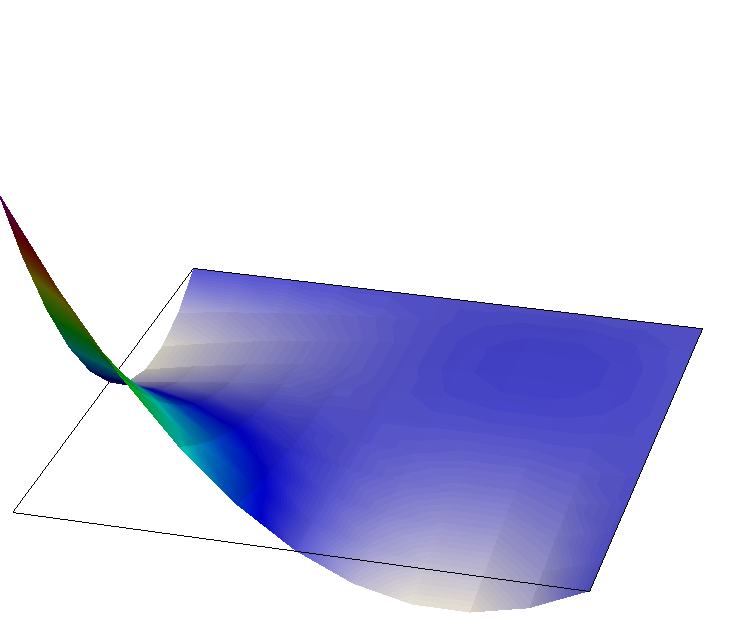
\includegraphics[width=.3\textwidth]{graph/shape0}
    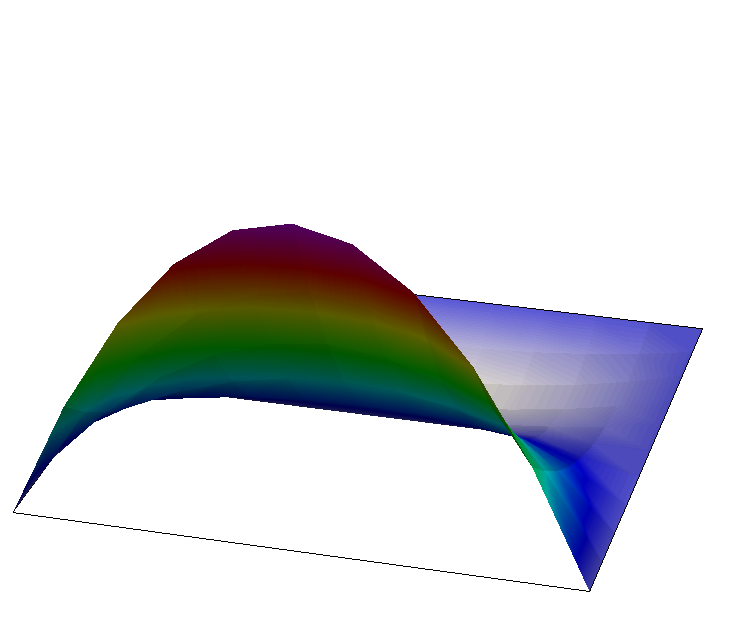
\includegraphics[width=.3\textwidth]{graph/shape1}
    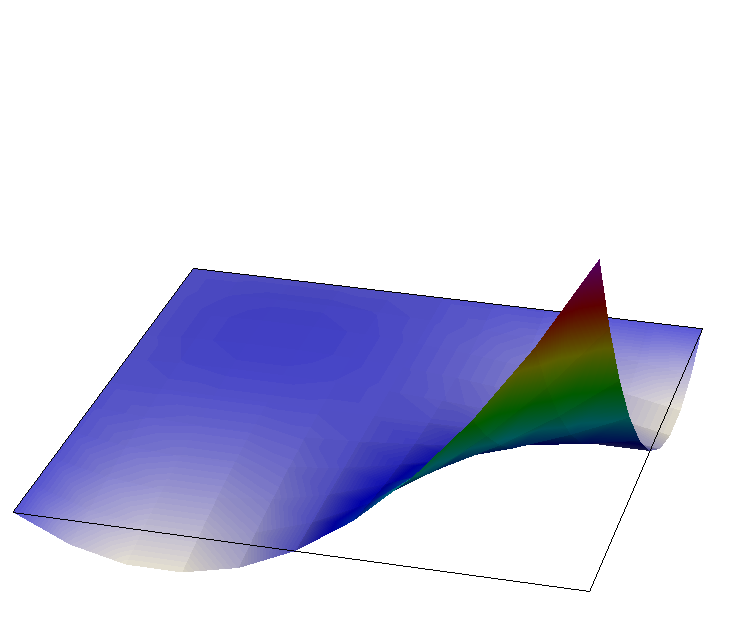
\includegraphics[width=.3\textwidth]{graph/shape2}

    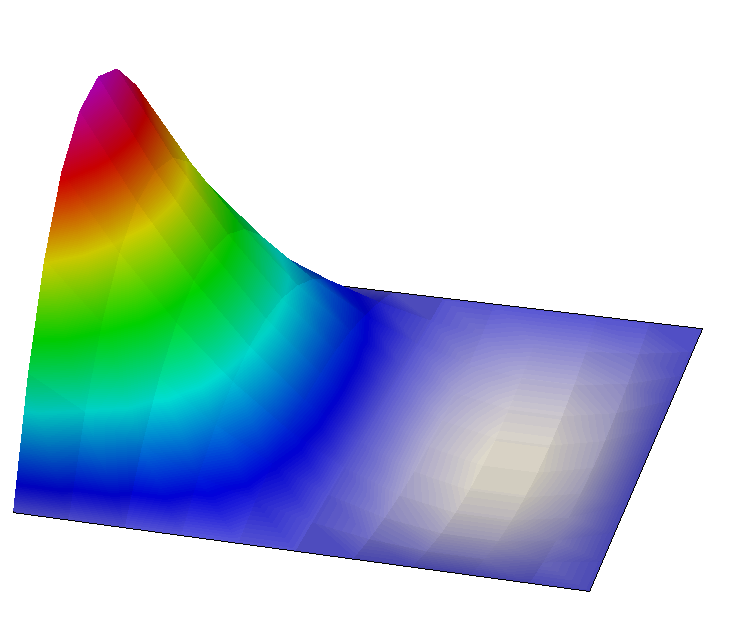
\includegraphics[width=.3\textwidth]{graph/shape3}
    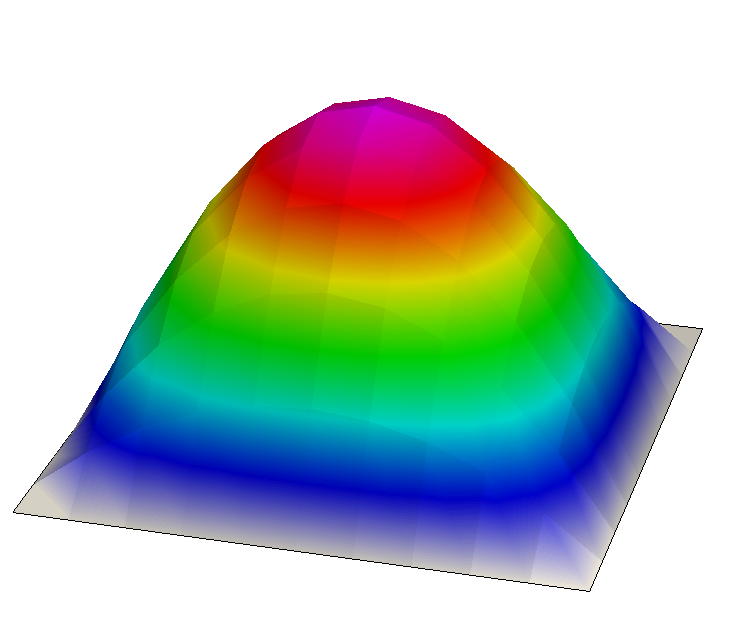
\includegraphics[width=.3\textwidth]{graph/shape4}
    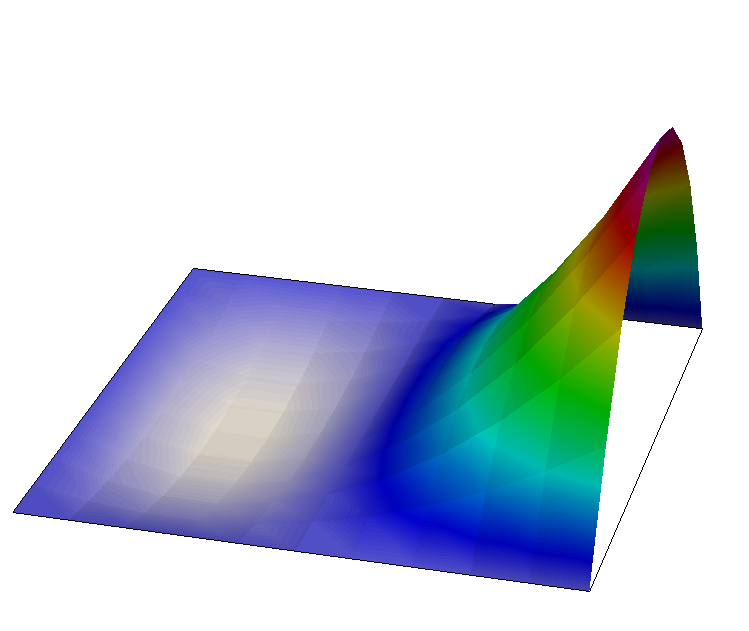
\includegraphics[width=.3\textwidth]{graph/shape5}

    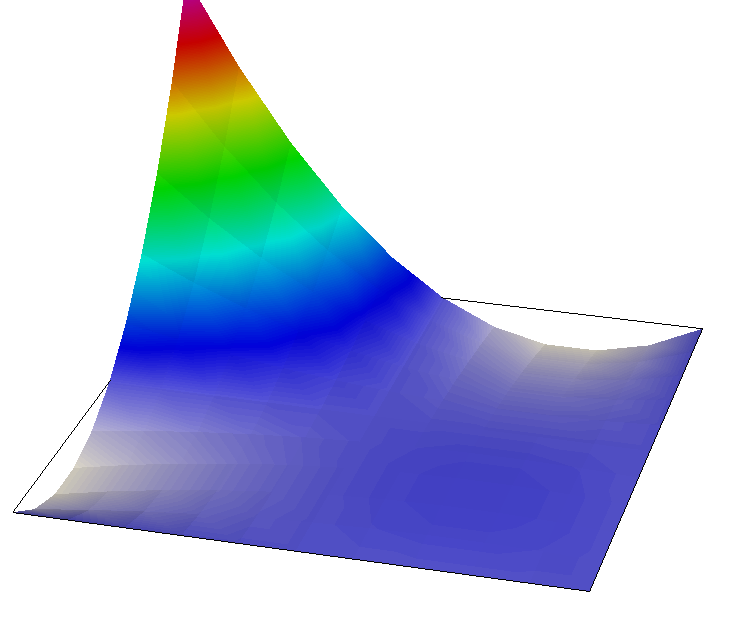
\includegraphics[width=.3\textwidth]{graph/shape6}
    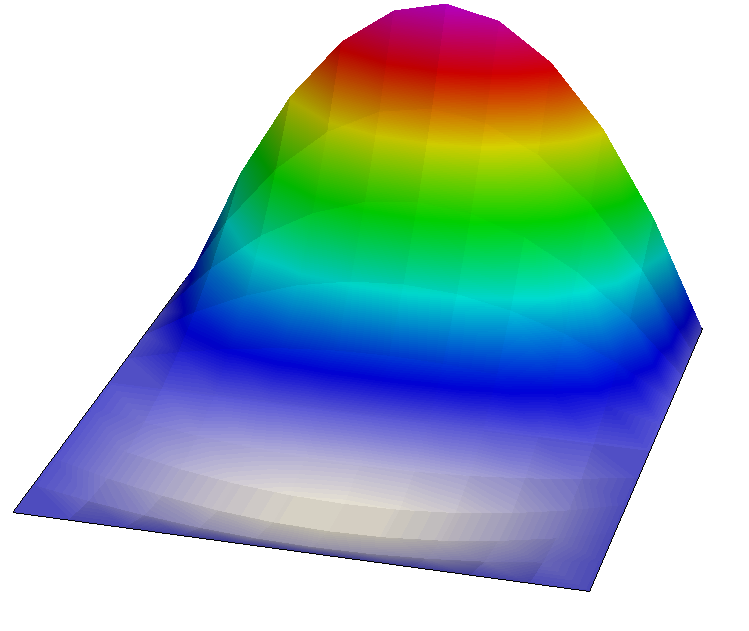
\includegraphics[width=.3\textwidth]{graph/shape7}
    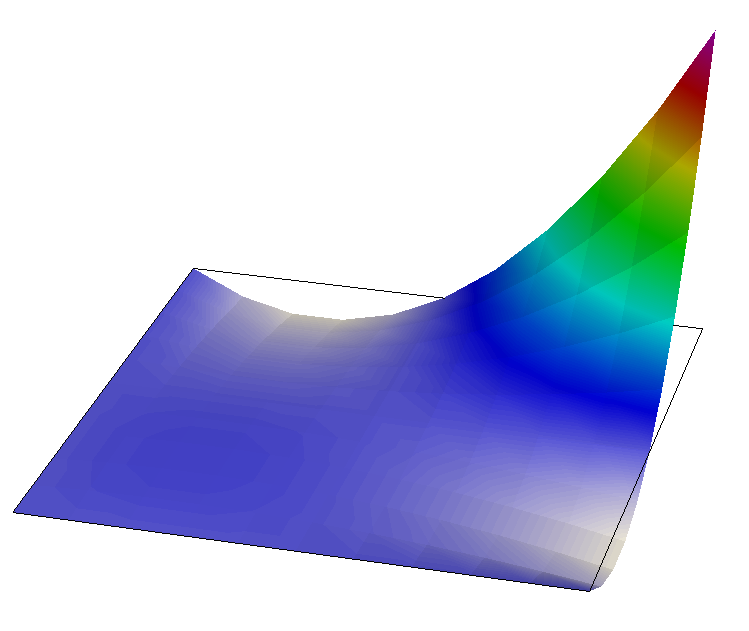
\includegraphics[width=.3\textwidth]{graph/shape8}
  \end{center}
\end{Example*}


\begin{Lemma}{tensor-product-trace}
  The trace of the $d$-dimensional tensor product polynomial space
  $\Q_k$ on the $\delta$-dimensional facets of the reference cube
  $\refcell = (0,1)^d$ is the $\delta$-dimensional space $\Q_k$.

  The traces from two cells sharing the same face coincide, if the
  mapping is continuous. Therefore, continuity can be achieved by
  unisolvent sets of node functionals on the face.
\end{Lemma}

\begin{proof}
  By keeping $d-\delta$ variables constant in the tensor product basis
  in~\eqref{eq:fem-intro:1}.
\end{proof}

\begin{Example*}{cg-q2}{Continuous basis functions}
  \begin{center}
    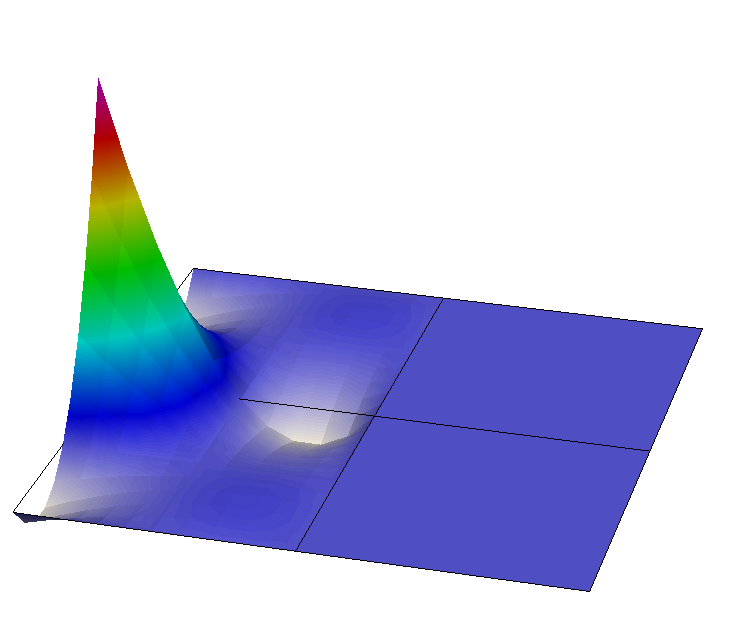
\includegraphics[height=.20\textwidth]{graph/cgbasis1-02}
    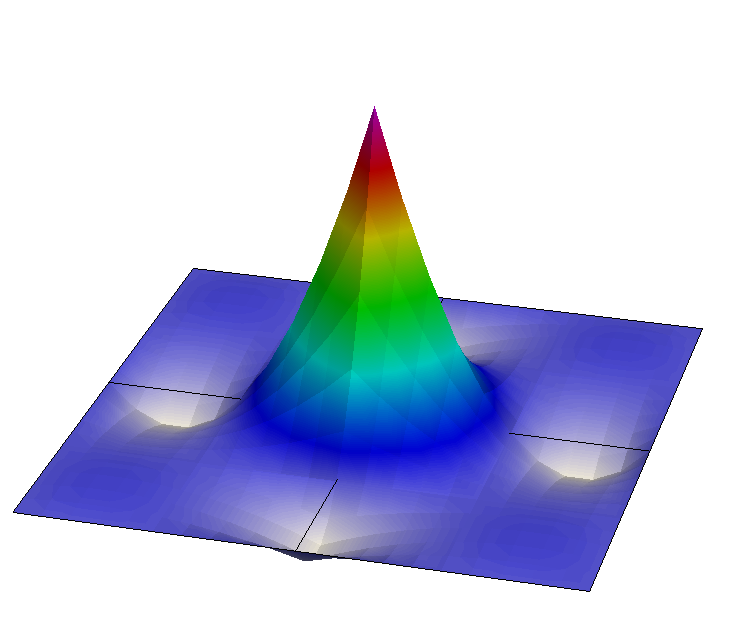
\includegraphics[height=.20\textwidth]{graph/cgbasis1-03}
    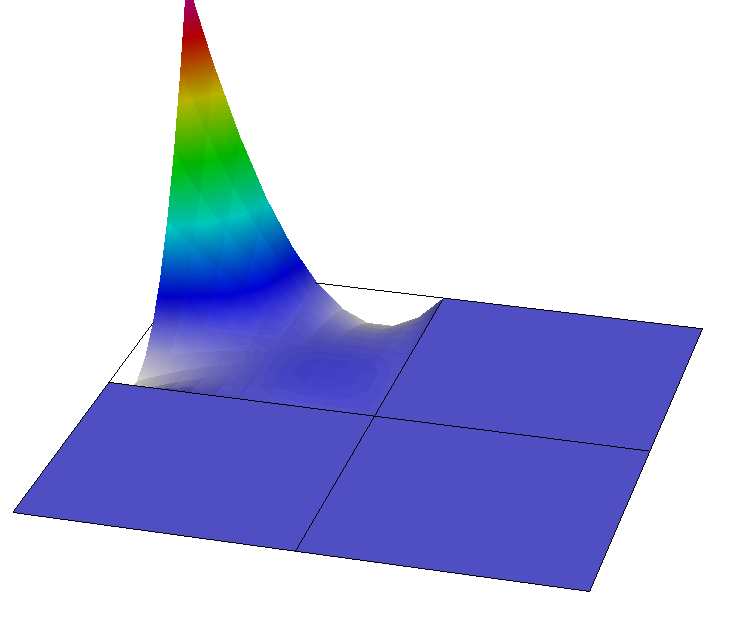
\includegraphics[height=.20\textwidth]{graph/cgbasis1-15}
    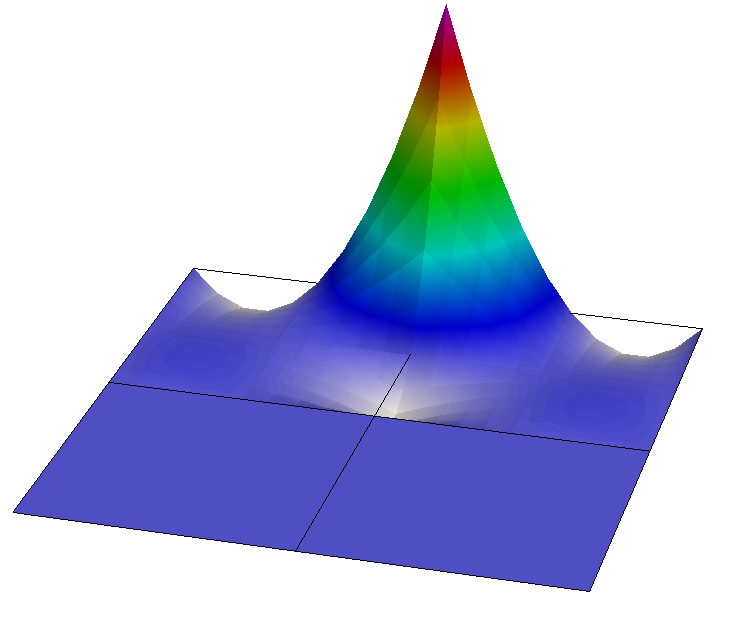
\includegraphics[height=.20\textwidth]{graph/cgbasis1-16}

    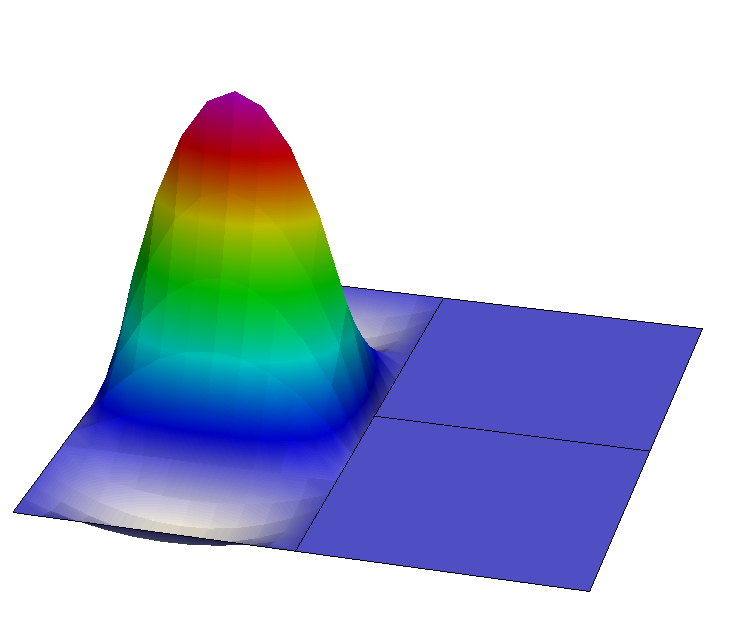
\includegraphics[height=.20\textwidth]{graph/cgbasis1-07}
    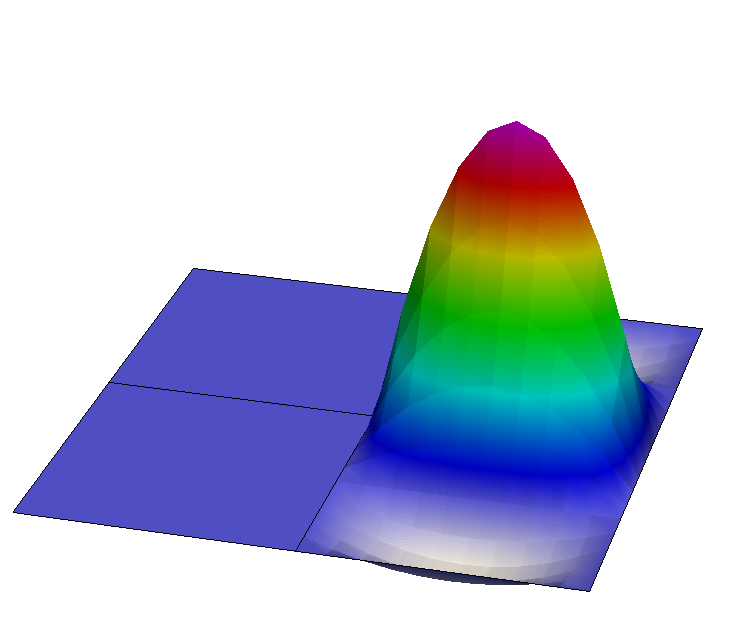
\includegraphics[height=.20\textwidth]{graph/cgbasis1-13}
    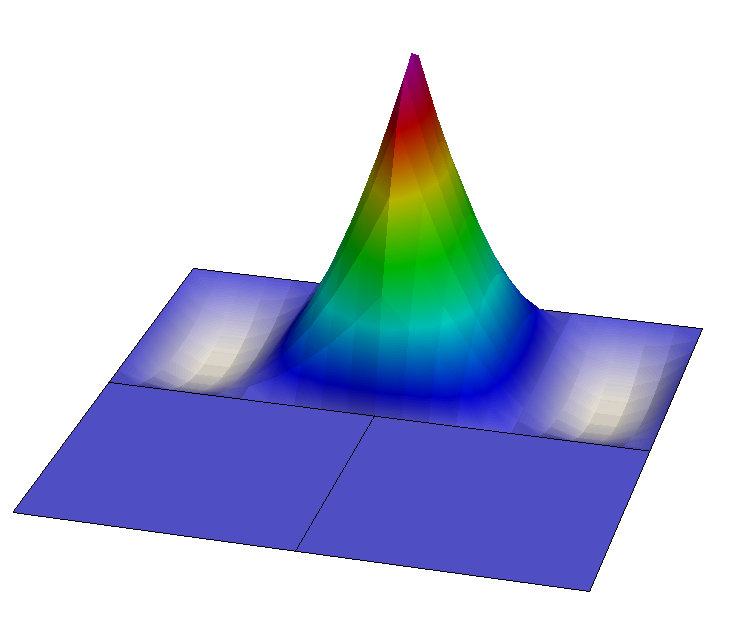
\includegraphics[height=.20\textwidth]{graph/cgbasis1-18}
    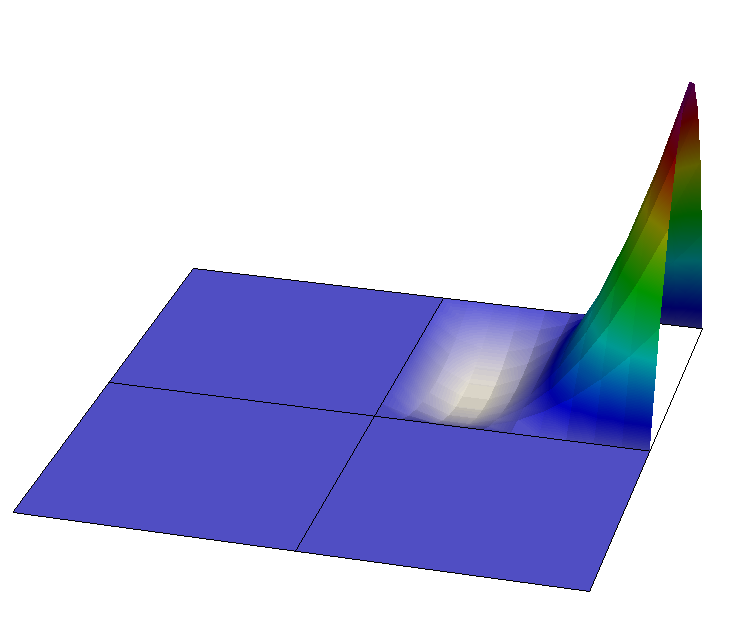
\includegraphics[height=.20\textwidth]{graph/cgbasis1-22}

    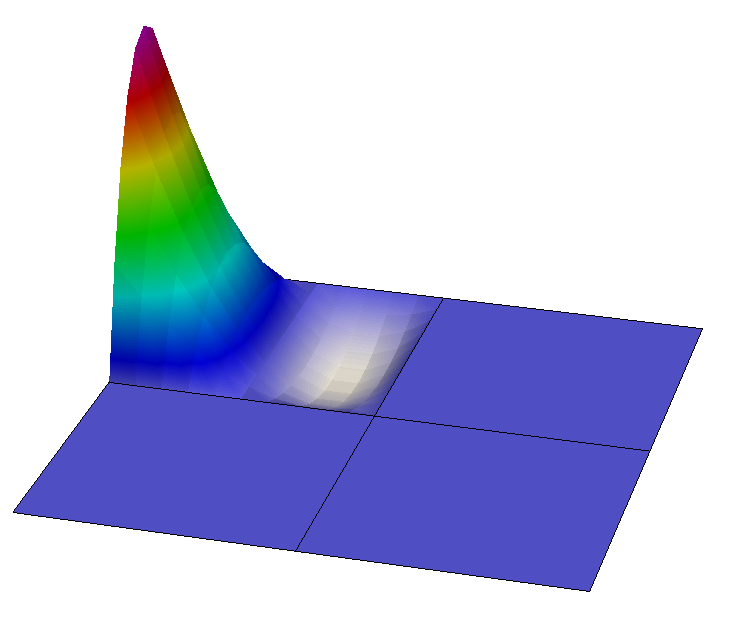
\includegraphics[height=.20\textwidth]{graph/cgbasis1-17}
    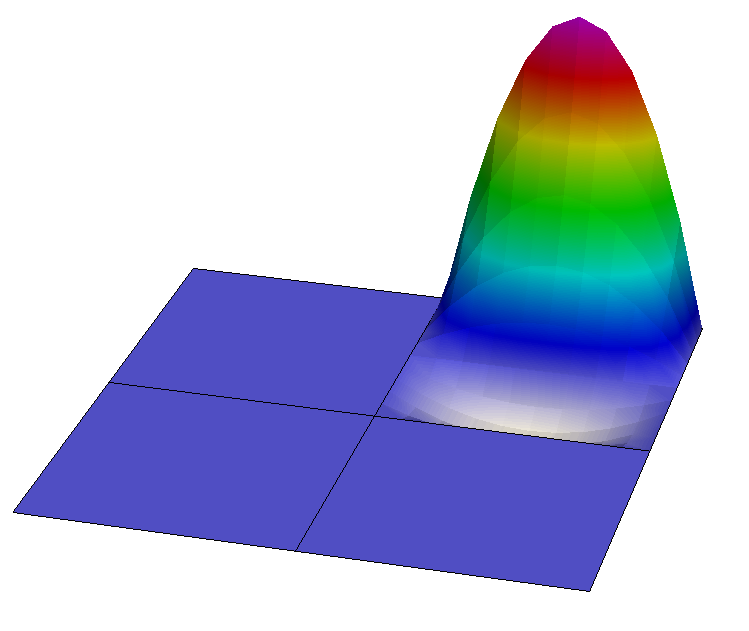
\includegraphics[height=.20\textwidth]{graph/cgbasis1-23}
    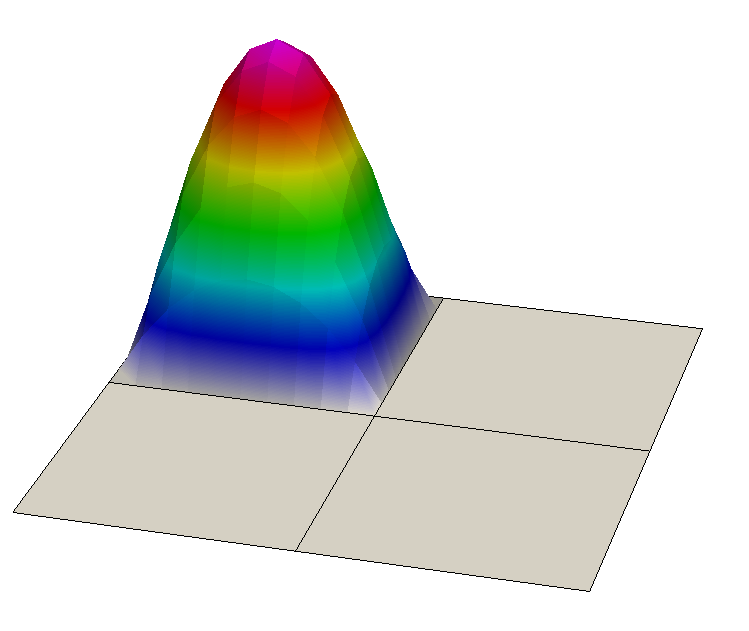
\includegraphics[height=.20\textwidth]{graph/cgbasis1-20}
    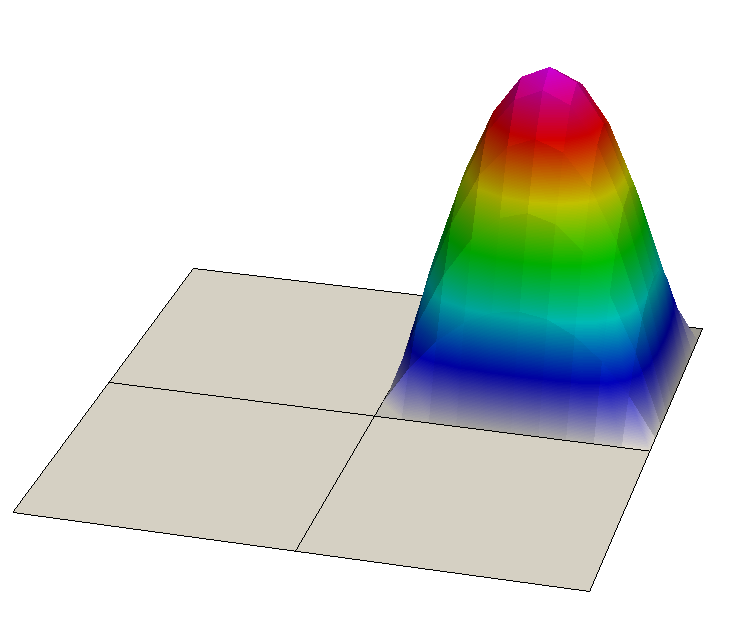
\includegraphics[height=.20\textwidth]{graph/cgbasis1-24}
  \end{center}
\end{Example*}

\begin{Example*}{dg-q2}{Discontinuous basis functions}
  \begin{center}
    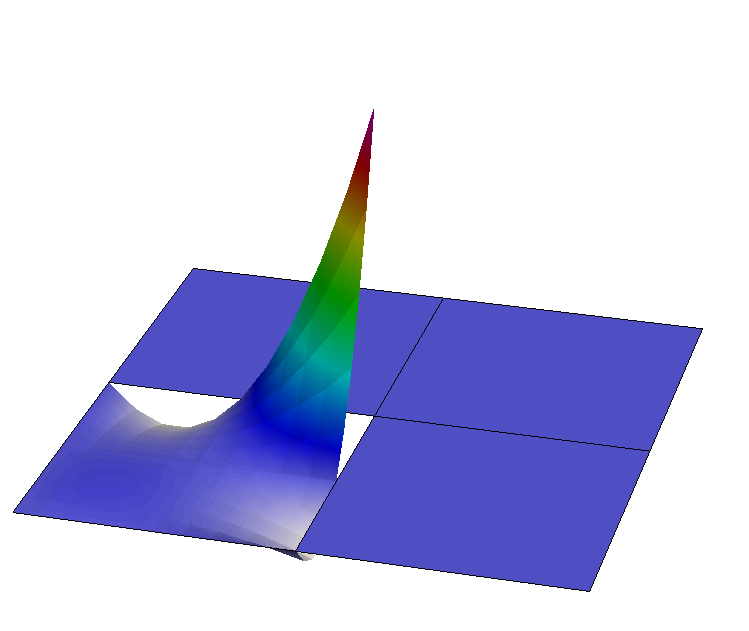
\includegraphics[height=.20\textwidth]{graph/dgbasis1-08}
    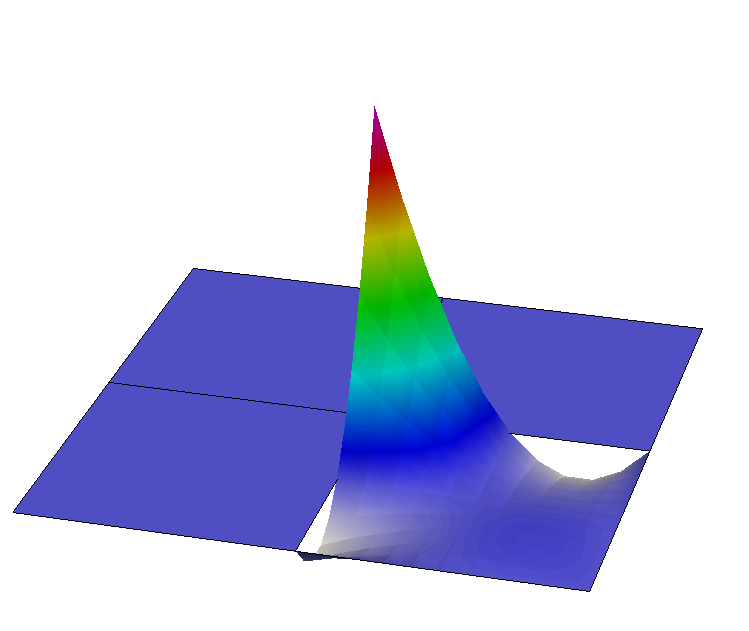
\includegraphics[height=.20\textwidth]{graph/dgbasis1-15}
    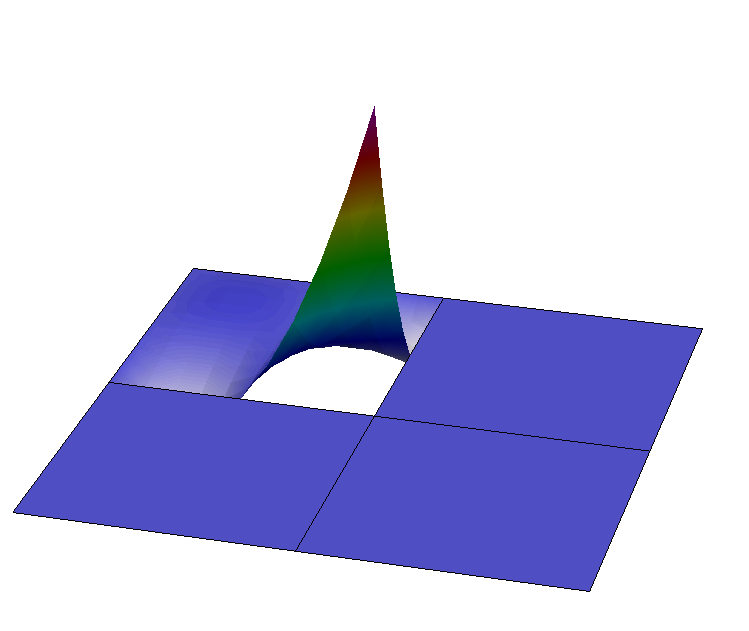
\includegraphics[height=.20\textwidth]{graph/dgbasis1-20}
    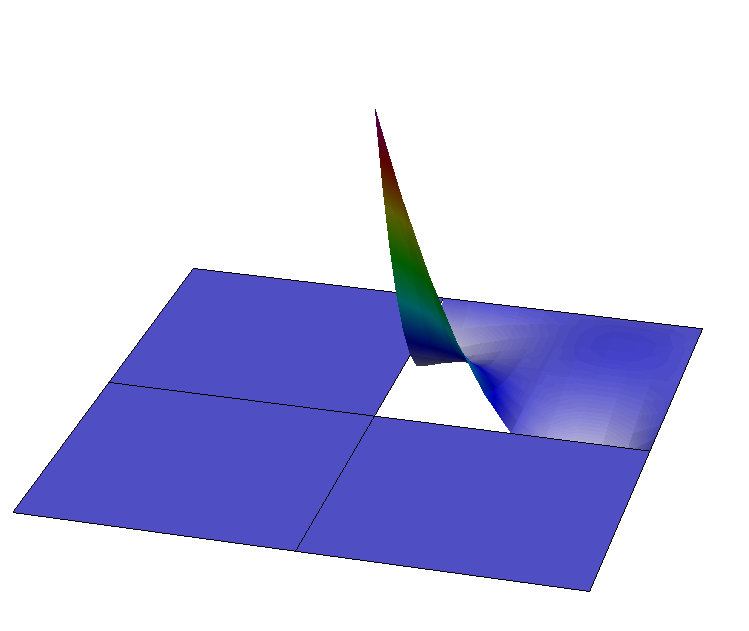
\includegraphics[height=.20\textwidth]{graph/dgbasis1-27}

    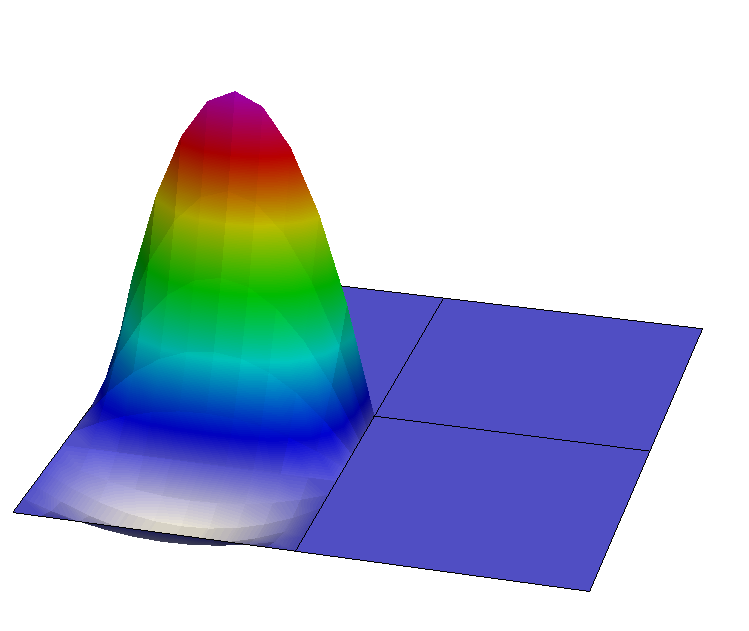
\includegraphics[height=.20\textwidth]{graph/dgbasis1-07}
    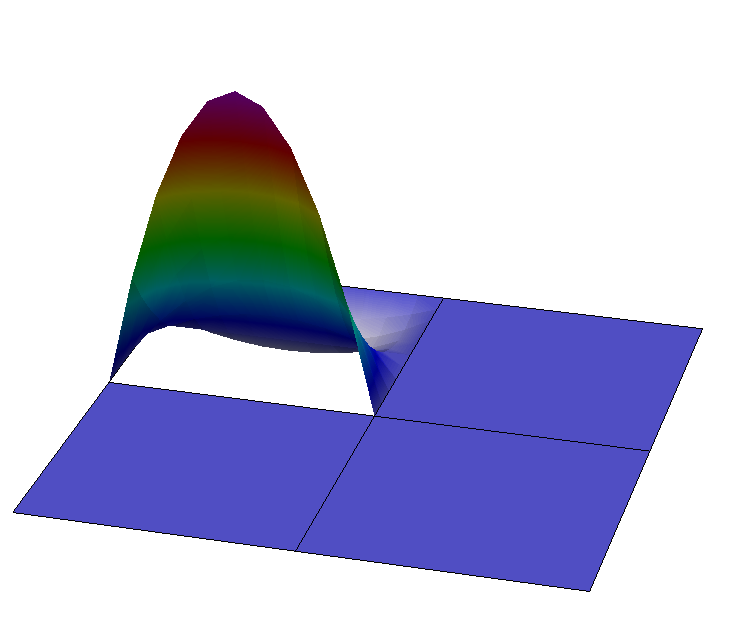
\includegraphics[height=.20\textwidth]{graph/dgbasis1-19}
    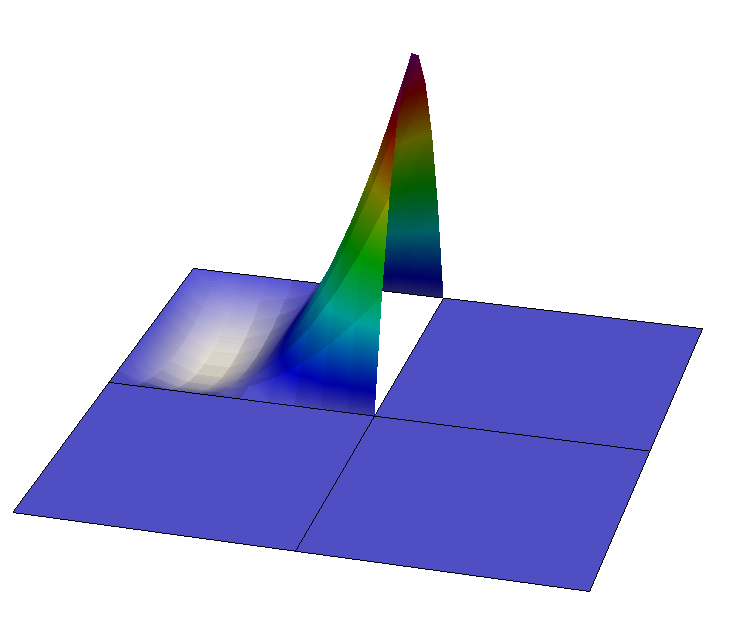
\includegraphics[height=.20\textwidth]{graph/dgbasis1-23}
    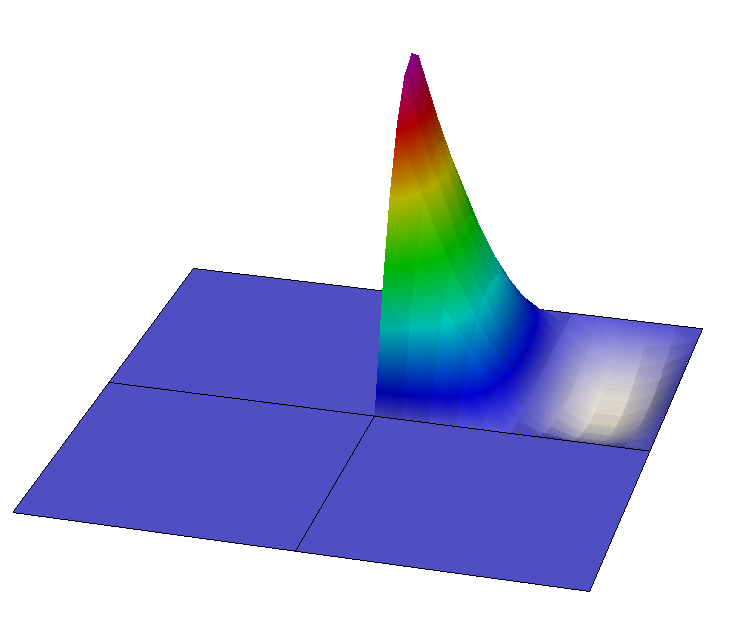
\includegraphics[height=.20\textwidth]{graph/dgbasis1-30}

    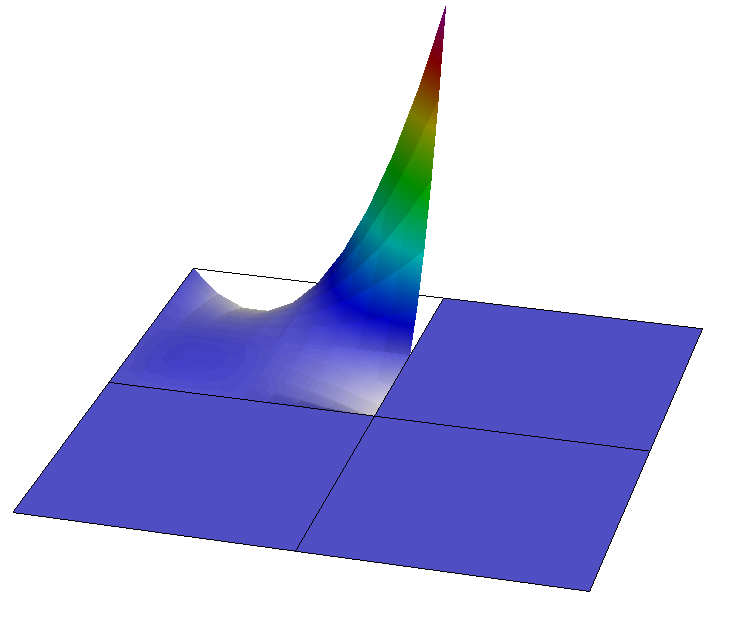
\includegraphics[height=.20\textwidth]{graph/dgbasis1-26}
    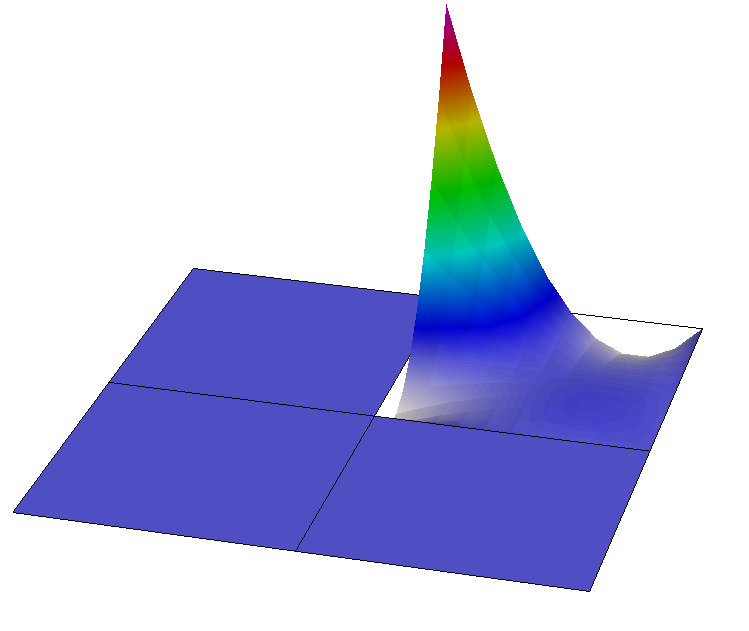
\includegraphics[height=.20\textwidth]{graph/dgbasis1-33}
    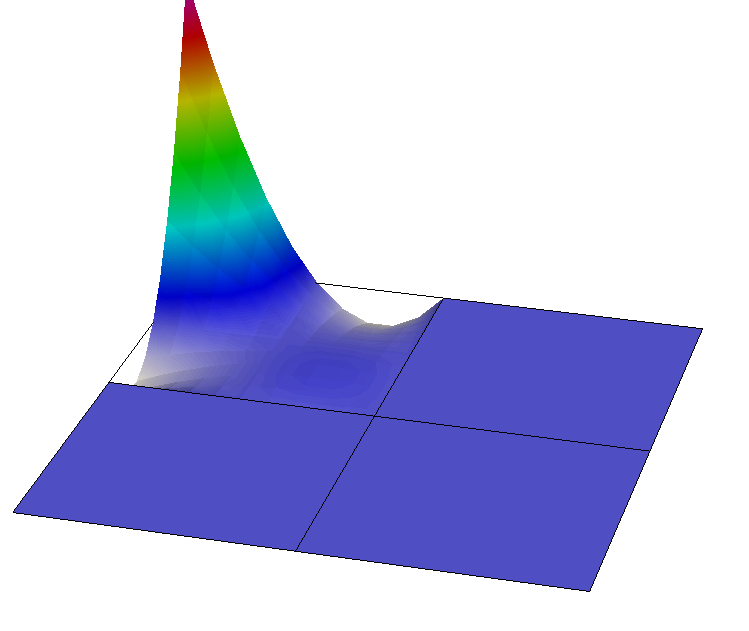
\includegraphics[height=.20\textwidth]{graph/dgbasis1-24}
    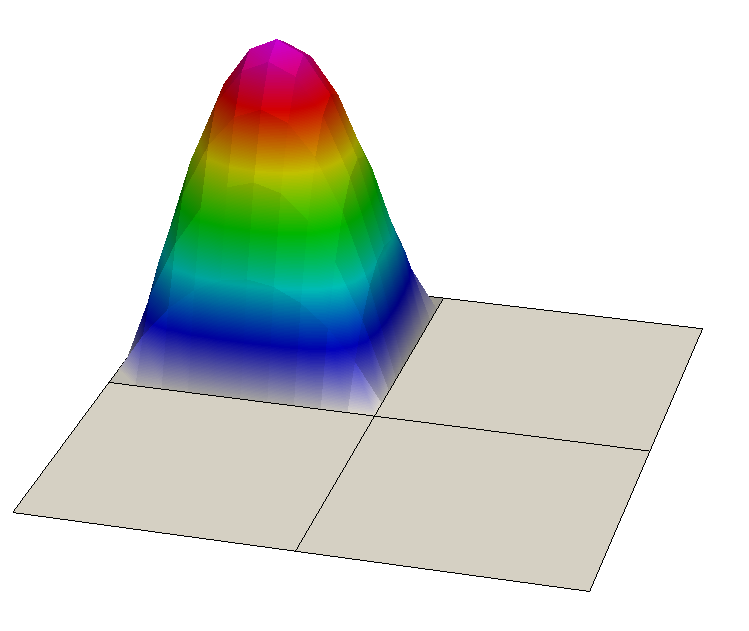
\includegraphics[height=.20\textwidth]{graph/dgbasis1-22}
  \end{center}
\end{Example*}

\begin{example}
  As a second example, we choose $d=2$ and the univariate space $\P_2$ with node functionals
  \begin{gather}
    \nodal_0(p) = p(0),
    \quad \nodal_1(p) = \int_0^1 p(t) \dt,
    \quad \nodal_2(p) = p(1),
  \end{gather}
  that is, a mixture of Lagrange interpolation and orthogonality on
  the interval $[0,1]$. The matching basis polynomials are
  \begin{gather}
    p_0(t) = 3(1-t)^2 - 2(1-t),
    \quad p_1(t) = 6 t(1-t),
    \quad p_2(t) = 3t^2-2t.
  \end{gather}
  Follwoing the construction of the previous example, we obtain
  \begin{gather}
    \begin{aligned}
    \nodal_{00}(p) &= p(0,0),
    &\nodal_{02}(p) &= p(0,1),\\
    \nodal_{20}(p) &= p(1,0),
    &\nodal_{22}(p) &= p(1,1).
    \end{aligned}
  \end{gather}
  Then,
  \begin{gather}
    \nodal_{01}(p_{01}) = \nodal_{01}(p_0\otimes p_1)
    = p_0(0)\int_0^1 p_1(y)\dy
    = \int_0^1 p(0,y) \dy.
  \end{gather}
  Thus, the node functional $\nodal_{01}$ is the integral over the
  left edge of the reference square. By the same construction,
  $\nodal_{01}$ is the integral over the right edge. $\nodal_{10}$ and
  $\nodal_{12}$ are the integrals over the bottom and top edge,
  respectively. Finally,
  \begin{gather}
    \nodal_{11}(p_{11})
    = \int_0^1 p_1(x)\dx \int_0^1 p_1(y) \dy
    = \int_0^1\int_0^1 p_{11}(x,y) \dx\dy.
  \end{gather}
  Thus, the tensor product of two line integrals becomes the integral
  over the area.
\end{example}



%%%%%%%%%%%%%%%%%%%%%%%%%%%%%%%%%%%%%%%%%%%%%%%%%%%%%%%%%%%%%%%%%%%%%%
%%%%%%%%%%%%%%%%%%%%%%%%%%%%%%%%%%%%%%%%%%%%%%%%%%%%%%%%%%%%%%%%%%%%%%
\subsection{The Galerkin equations and Céa's lemma}
%%%%%%%%%%%%%%%%%%%%%%%%%%%%%%%%%%%%%%%%%%%%%%%%%%%%%%%%%%%%%%%%%%%%%%
%%%%%%%%%%%%%%%%%%%%%%%%%%%%%%%%%%%%%%%%%%%%%%%%%%%%%%%%%%%%%%%%%%%%%%

\begin{Definition*}{galerkin-approximation}{Galerkin approximation}
  Let $u\in V$ be determined by the weak formulation
  \begin{gather*}
    a(u,v) = f(v) \qquad\forall v\in V,
  \end{gather*}
  where $V$ is a suitable function space including boundary
  conditions. The \define{Galerkin approximation}, also called
  \define{conforming approximation} of this problem reads as follows:
  choose a subspace $V_n\subset V$ of dimension $n$ and find
  $u_n\in V_n$, such that
  \begin{gather*}
    a(u_n,v_n) = f(v_n) \qquad\forall v_n\in V_n.
  \end{gather*}
  We will refer to this equation as the \define{discrete problem}.
\end{Definition*}

\begin{Corollary*}{galerkin-equations}{Galerkin equations}
  After choosing a basis $\{v_i\}$ for $V_n$, the Galerkin equations are
  equivalent to a linear system
  \begin{gather}
    \mata \vu = \vf,
  \end{gather}
  with $\mata\in\R^{n\times n}$ and $\vf\in \R^n$ defined by
  \begin{gather}
    a_{ij} = a(v_j, v_i), \qquad f_i = f(v_i).
  \end{gather}
\end{Corollary*}

\begin{Lemma}{discrete-lax-milgram}
  If the lemma of Lax-Milgram holds for $a(.,.)$ on $V$, it holds on
  $V_n\subset V$. In particular, solvability of the Galerkin equations
  is implied.
\end{Lemma}

\begin{proof}
  Since coercivity and boundedness hold for all $u,v\in V$ they hold
  in particular for all $u,v\in V_n$.
\end{proof}

\begin{Lemma}{galerkin-ortho}
  Let $a(.,.)$ be a bilinear form on the Hilbert
  space $V$.
  Let $u \in V$ and $u_n\in V_n \subset V$ be the solution to the
  weak formulation and its Galerkin approximation
  \begin{gather*}
    \begin{aligned}
      a(u,v) &= f(v) & \qquad\forall v&\in V,\\
      a(u_n,v_n) &= f(v_n) & \qquad\forall v_n&\in V_n,
    \end{aligned}
  \end{gather*}
  respectively. Then, there holds the \define{Galerkin orthogonality}
  \begin{align}
    \label{eq:galerkin-ortho}
    a(u-u_n,v_n) = 0 \qquad \forall v_n\in V_n.
  \end{align}
\end{Lemma}

\begin{proof}
  As $v_n\in V_n$ there holds $a(u,v_n)=f(v_n)$, too.
  Then, there holds for an arbitrary $v_n\in V_n$
  \begin{gather*}
    a(u-u_n,v_n)=a(u,v_n)-a(u_n,v_n)=f(v_n)-f(v_n)=0.
  \end{gather*}
\end{proof}

\begin{Lemma*}{cea}{Céa}
  Let $a(.,.)$ be a bounded and elliptic bilinear form on the Hilbert
  space $V$.  Let $u \in V$ and $u_n\in V_n \subset V$ be
  the solution to the weak formulation and its Galerkin approximation
  respectively. Then, there holds
  \begin{gather}
    \norm{u-u_n}_V \le \frac{M}{\alpha}
    \inf_{v_n\in V_n}\norm{u-v_n}_V.
  \end{gather}
\end{Lemma*}

\begin{proof}
  As $a(.,.)$ is coercive with $\alpha>0$ and bounded with $M>0$
  we get for arbitrary $v_n\in V_n$
  \begin{gather*}
    \begin{aligned}
      \alpha \norm{u-u_n}_V^2 &\le a(u-u_n,u-u_n) = a(u-u_n,u-v_n+v_n-u_n) \\
      &= a(u-u_n,u-v_n) + \underbrace{a(u-u_n,v_n-u_n)}_{=0} \\
      &\le M \norm{u-u_n}_V \norm{u-v_n}_V.
    \end{aligned}
  \end{gather*}
  In the second line we applied the Galerkin orthogonality
  as $v_n-u_n\in V_n$. Dividing by $\norm{u-u_n}_V$ there holds
  \begin{gather*}
    \norm{u-u_n}_V \leq \frac{M}{\alpha} \norm{u-v_n}_V.
  \end{gather*}
  As $v_n\in V_n$ was chosen arbitrary, we conclude
  \begin{gather*}
    \norm{u-u_n}_V \le \inf_{v_n\in V_n} \norm{u-v_n}_V.
  \end{gather*}
\end{proof}

\begin{Lemma}{fe-matrix}
  For a finite element discretization of Poisson's equation with the
  space $V_\mesh$, the Galerkin equations can be computed using the
  following formulas:
  \begin{alignat*}3
    a_{ij} &= \int\limits_\domain \nabla v_j \cdot \nabla v_i \dx
    &&= \int\limits_{\domain(\nodal^i)} \nabla v_j \cdot \nabla v_i \dx
    &&= \sum_{\cell\in\mesh(\nodal^i)}\int\limits_\cell \nabla v_j \cdot \nabla v_i \dx\\
    f_{i} &= \int\limits_\domain f v_i \dx
    &&= \int\limits_{\domain(\nodal^i)} f v_i \dx
    &&= \sum_{\cell\in\mesh(\nodal^i)}\int\limits_\cell f v_i \dx
  \end{alignat*}
\end{Lemma}

\begin{Algorithm*}{matrix-assembling}{Assembling the matrix}
  \begin{enumerate}
  \item Start with a matrix $\mata = 0 \in \R^{n\times n}$
  \item Loop over all cells $\cell\in\mesh$
  \item On each cell $\cell$, compute a cell matrix
    $\mata_\cell \in \R^{n_\cell\times n_\cell}$ by integrating
    \begin{gather}
      a_{\cell,ij} = \int_\cell \nabla p_{\cell,j}\cdot\nabla p_{\cell,i}\,dx,
    \end{gather}
    where $\{p_{\cell,i}\}$ is the shape function basis.
  \item Assemble the cell matrices into the global matrix by
    \begin{gather}
      a_{\iota(i),\iota(j)} = a_{\iota(i),\iota(j)} + a_{\cell,ij}
      \qquad i,j = 1,\dots,n_\cell.
    \end{gather}
  \end{enumerate}
\end{Algorithm*}

%%%%%%%%%%%%%%%%%%%%%%%%%%%%%%%%%%%%%%%%%%%%%%%%%%%%%%%%%%%%%%%%%%%%%%
%%%%%%%%%%%%%%%%%%%%%%%%%%%%%%%%%%%%%%%%%%%%%%%%%%%%%%%%%%%%%%%%%%%%%%
\subsection{Mapped finite elements}
%%%%%%%%%%%%%%%%%%%%%%%%%%%%%%%%%%%%%%%%%%%%%%%%%%%%%%%%%%%%%%%%%%%%%%
%%%%%%%%%%%%%%%%%%%%%%%%%%%%%%%%%%%%%%%%%%%%%%%%%%%%%%%%%%%%%%%%%%%%%%

\begin{Definition}{mapped-mesh}
  A mapped mesh $\mesh$ is a set of cells $\cell$, which are defined
  by a single \define{reference cell} $\refcell$ and individual
  smooth mappings
  \begin{gather}
    \begin{split}
      \Phi_\cell \colon \refcell &\to \R^d\\
      \Phi_\cell(\refcell) &= \cell.
    \end{split}
  \end{gather}
  The definition extends to small sets of reference cells, for
  instance for triangles and quadrilaterals.
\end{Definition}

\begin{Example}{mapping-linear}
  Let the reference triangle $\refcell$ be defined by
  \begin{gather}
    \refcell = \left\{
      \begin{pmatrix}
        \refx\\\refy
      \end{pmatrix}
      \middle|
      \refx,\refy >0, \refx+\refy < 1
    \right\}.
  \end{gather}
  Then, every cell $\cell$ spanned by the vertices $\vertex_0$,
  $\vertex_1$, and $\vertex_2$ is obtained by mapping $\refcell$ by
  the \putindex{affine mapping}
  \begin{gather}
    \Phi_\cell(\refvx) =
    \begin{pmatrix}
      X_1-X_0 & X_2 - X_0 \\ Y_1-Y_0 & Y_2 - Y_0
    \end{pmatrix}
    \begin{pmatrix}
      \refx \\ \refy
    \end{pmatrix}
    +
    \begin{pmatrix}
      X_0 \\ Y_0
    \end{pmatrix} =: \matb_\cell \refvx + \vb_\cell
  \end{gather}
\end{Example}

\begin{Example}{mapping-bilinear}
  The reference cell for a quadrilateral is the reference square
  $\refcell = (0,1)^2$. Every quadrilateral $\cell$ spanned by the
  vertices $\vertex_0$ to $\vertex_3$ is then obtained by the
  \putindex{bilinear mapping}
  \begin{gather}
    \Phi_\cell(\refvx)
    = \vertex_0 (1-\refx)(1-\refy)
    + \vertex_1 \refx(1-\refy)
    + \vertex_2 (1-\refx)\refy
    + \vertex_3 \refx\refy
  \end{gather}
\end{Example}

\begin{Definition}{mapped-fe}
  Mapped shape functions $\{p_i\}$ on a mesh cell $\cell$ are defined by a
  set of shape functions $\{\refp_i\}$ on the reference cell
  $\refcell$ through \define{pull-back}
  \begin{gather}
    \begin{split}
      p_i(\vx) &= \refp_i\left(\Phi^{-1}(\vx)\right) = \refp_i(\refvx),\\
      \nabla p_i(\vx) &= \nabla\Phi^{-T}(\refvx)\refgrad\refp_i(\refvx)
    \end{split}
  \end{gather}
\end{Definition}

\begin{Lemma}{mapped-norms-affine}
  Let $\refcell$ be the reference triangle and let $\cell$ be a
  triangular mesh cell with mapping
  $\vx = \Phi_\cell(\refvx) = \matb \refvx + \vb$. Let there hold
  $u(\vx) = \refu(\refvx)$. Then, $u\in H^k(\cell)$ if and only if
  $\refu\in H^k(\refcell)$ and we have with some constant $c$ the
  estimates
  \begin{gather}
    \begin{split}
      \snorm{\refu}_{k,\refcell}
      &\le c \norm{\matb}^k (\det \matb)^{-\nicefrac12}
      \snorm{u}_{k,\cell},\\
      \snorm{u}_{k,\cell}
      &\le c \norm{\matb^{-1}}^k (\det \matb)^{\nicefrac12}
      \snorm{\refu}_{k,\refcell}.
    \end{split}
  \end{gather}
\end{Lemma}

\begin{Lemma}{shape-regular-transformation}
  For a cell $\cell$, let $R$ be the radius of the circumscribed
  circle and $\rho$ the radius of the inscribed circle. Then,
  \begin{gather}
    \norm{\matb} \le c R, \qquad \norm{\matb^{-1}} \le c \rho^{-1}.
  \end{gather}
\end{Lemma}

\begin{proof}
  \begin{figure}
    \centering
    \begin{tikzpicture}
    \def\scale{3}
    
    %% reference cell
    \def\mid{\scale*0.2928932188}
    \def\outermid{\scale*0.5}
    \def\outerrad{\scale*0.7071067811}
    
    \node (mid) at (\mid,\mid) {$\refvx_0$};
    \coordinate (x1) at (\scale*1,0);
    \node[right = \scale*0.01 of x1] (x1name) {$\refvx_1$};
    \coordinate (x2) at (0,\scale*1);
    \node[above = \scale*0.01 of x2] (x2name) {$\refvx_2$};
    \coordinate (x3) at (0,0);
    \node[left = \scale*0.01 of x3] (x3name) {$\refvx_3$};
    \coordinate (xc) at (\outermid,\outermid);
    \node[above = \scale*0.01 of xc] (xcname) {$\refvx_c$};
    
    \draw (x1)--(x2)--(x3)--(x1);
    
    % incircle
    \draw (mid) circle (\mid);
    \draw (mid) --  (\mid,0);
    \node[below = \scale*0.01 of mid,xshift=0.5em] (rho) {$\refrho$};
    
    % circumcircle
    \draw (xc) circle (\outerrad);
    \draw (xc) -- (\outermid+\outerrad,\outermid);
    \node[above right = \scale*0.01 and \scale*0.25 of xc] (R) {$\reference{R}$};
    \end{tikzpicture}
    \caption{Visualization of the inscribed and circumscribed circle of the reference cell $\refcell$.}
  \end{figure}

  Let us define $S_{\refrho}\coloneqq \{\refvy\in\R^d ~\mid~ \abs{\refvy}=\refrho \}$.
  For $\refvy\in S_{\refrho}$ there holds
  $\refvx\coloneqq \refvxo + \refvy\in \overline{\refcell}$
  and $\vx=\matb\refvx + \vb = \matb(\refvxo+\refvy)+\vb$.
  Additionally, we have $\vxo = \matb \refvxo + \vb$
  which yields
  \begin{align*}
    \abs{\vx-\vxo} = \abs{\matb\refvy}\leq 2R.
  \end{align*}
  Now consider the operator norm of $\matb$
  \begin{align*}
    \norm{\matb} = \sup_{\refvy\in\R^d} \frac{\abs{\matb\refvy}}{\abs{\refvy}}
    = \sup_{\abs{\refvy}=1} \abs{\matb\refvy}
    = \sup_{\refvy\in S_{\refrho}} \frac{\abs{\matb\refvy}}{\refrho}
    \leq \frac{2R}{\refrho}.
  \end{align*}
  $\refrho$ is a constant only depending on $\refcell$ but
  not on $\cell$. Hence, we get $\norm{\matb}\leq cR$ with $c$ depending
  on $\refrho$.

  The same argument can be applied for the second estimate.
  We now define $S_\rho\coloneqq \{\vy\in\R^d~\mid~\abs{\vy}=\rho \}$.
  For $\vy\in S_\rho$ there holds $\vx\coloneqq\vxo+\vy\in\overline{\cell}$
  and let $\refvx=\matb^{-1}\vx-\vb,~\refvxo=\matb^{-1} \vxo - \vb$ which yields
  \begin{align*}
    \abs{\refvx - \refvxo} = \abs{\matb^{-1} \vy}\leq 2\reference{R}.
  \end{align*}
  Analogous to the first estimate we obtain
  \begin{align*}
    \norm{\matb^{-1}} = \sup_{\vy\in S_\rho} \frac{\abs{\matb^{-1} \vy}}{\rho}
    \leq \frac{2\reference{R}}{\rho}.
  \end{align*}
  Now $\reference{R}$ is only depending on $\refcell$ but not on $\cell$.
  Hence, we have $\norm{\matb^{-1}}\leq c\rho^{-1}$ where $c$ depends
  on $\reference{R}$.
\end{proof}

\begin{Assumption}{mapping-decomposition}
  For more general mappings $\Phi\colon \refcell\to \cell$, we
  make the assumption, that they can be decomposed into three factors,
  \begin{gather}
    \Phi = \Phi_O \circ \Phi_S \circ \Phi_W,
  \end{gather}
  where $\Phi_O$ is a combination of translation and rotation,
  $\Phi_S$ is a scaling with a characteristic length $h_T$, and
  $\Phi_W$ is a warping function not changing the characteristic length.
\end{Assumption}

\begin{example}
  We construct the inverse of $\Phi$ in two dimensions by the
  following three steps, using as $h_\cell$ the length of the longest
  edge of $\cell$.
  \begin{enumerate}
  \item Choose $\Phi_O$ as the rigid body movement which maps the
    longest edge to the interval $(0,h_\cell)$ on the $x$-axis and the
    cell itself to $\cell_O$ in the positive half plane. This mapping
    has the structure
    \begin{gather*}
      \Phi^{-1}_O (\vx) = \mats \vx - \mats \vertex_0,
    \end{gather*}
    where $\mats$ is an orthogonal matrix and $\vertex_0$ is the
    vertex moved to the origin.
  \item Choose the scaling
    \begin{gather*}
      \Phi^{-1}_S (\vx) = \tfrac1{h_\cell} \vx,
    \end{gather*}
    such that the longest edge of the resulting cell $\cell_S$ has the
    longest edge equal to the interval $(0,1)$ on the $x$-axis.
  \item Warp the cell $\cell_S$ into the reference cell $\refcell$ by
    the mapping $\Phi^{-1}_W$. This operation leaves the longest edge
    untouched. For triangles, it is the uniquely defined linear
    transformation mapping the vertex not on the longest edge to
    $(0,1)$. For quadrilaterals, it is a bilinear transformation.
  \end{enumerate}

  In the first step, we have assumed that the cell is convex, which is
  always true for triangles. For nonconvex quadrilaterals, it can be
  shown that the determinant of $\nabla\Phi$ changes sign inside the
  cell, such that these cells are not useful for computations.

  The idea of this decomposition is, that we separate mappings
  changing the position, size, and shape of the cells.
\end{example}

\begin{Lemma*}{scaling-1}{Scaling lemma}
  Let the typical length of a cell $\cell$ be $h_\cell$. Assume there
  are constants $0 < M_\cell, m_\cell, d_\cell, D_\cell$, such that
  \begin{gather}
    \begin{split}
      \norm{\nabla\Phi_W(\refvx)} \le M_\cell,
      \\
      \norm{\nabla\Phi_W^{-1}(\refvx)} \le m_\cell^{-1} ,
      \\
      d^2_\cell \le \det \nabla\Phi_W(\refx)) \le D^2_\cell.      
    \end{split}
  \end{gather}
  for all $\refvx\in\refcell$. Then, for $k=0,1$ and a constant $c$
  \begin{gather}
    \begin{split}
      \snorm{\refu}_{k,\refcell}
      &\le c \frac{M_\cell}{d_\cell}  h_\cell^{k-\nicefrac d2}
      \snorm{u}_{k,\cell},\\
      \snorm{u}_{k,\cell}
      &\le c \frac{D_\cell}{m_\cell} h_\cell^{\nicefrac d2-k}
      \snorm{\refu}_{k,\refcell}.
    \end{split}
  \end{gather}
  This extends to higher derivatives under assumptions on higher
  derivatives of $\Phi_\cell$.
\end{Lemma*}

\begin{proof}
  By the chain rule,
  $\nabla \Phi_T = \nabla \Phi_O \nabla \Phi_S \nabla \Phi_W$. By
  construction, $\nabla\Phi_O$ is an orthogonal matrix, such that
  \begin{gather*}
    \norm{\nabla\Phi_O} = \norm{\nabla\Phi_O^{-1}} = 1.
  \end{gather*}
  Since it preserves angles and lengths, $\det \nabla\Phi_O =
  1$. Since $\Phi_S$ is a multiple of the identity, we have
  \begin{gather*}
    \norm{\nabla\Phi_S} = h_\cell,
    \quad\norm{\nabla\Phi_S^{-1}} = \frac1{h_\cell},
    \quad\det\nabla\Phi_S = h_\cell^d.
  \end{gather*}
  By change of variables, we have
  \begin{gather*}
    \int_\cell u^2 \dvx
    = \int_{\refcell} \refu^2 \abs{\det\nabla\Phi_\cell} \dvxref
    = \int_{\refcell} \refu^2 \det\nabla\Phi_S\det\nabla\Phi_O\det\nabla\Phi_W \dvxref
    ,
  \end{gather*}
  such that the case $k=0$ is proven immediately by
  \begin{gather*}
    h_T^d d_\cell^2 \int_{\refcell} \refu^2 \dvxref
    \le \int_\cell u^2 \dvx
    \le h_T^d D_\cell^2 \int_{\refcell} \refu^2 \dvxref
  \end{gather*}
  By the chain rule, we have
  \begin{gather*}
    \refgrad\refu(\refvx) = \nabla\Phi^T \nabla u(\vx)
    = \nabla\Phi_W^T \nabla\Phi_S^T \nabla\Phi_O^T \nabla u(\vx),
  \end{gather*}
  such that there holds
  \begin{gather}
    \begin{split}
      \abs{\refgrad\refu(\refvx)}
      &\le \norm{\nabla\Phi_W} h_\cell \abs{\nabla u},\\
      \abs{\nabla u(\vx)}
      &\le \norm{\nabla\Phi_W^{-1}} h_\cell^{-1} \abs{\refgrad \refu}.
    \end{split}
  \end{gather}
\end{proof}


\begin{Remark}{simple-mappings}
  We have $d_\cell = D_\cell$, if and only if the mapping is
  affine. The quotient $M_\cell/m_\cell$ measures how much the shape
  of the mesh cell deviates from the reference cell. For instance, it
  is one for squares.
\end{Remark}

%%% Local Variables: 
%%% mode: latex
%%% TeX-master: "main"
%%% End: 


%\chapter{Discontinuous Galerkin methods}
%\section{Nitsche's method}
%\label{sec:nitsches-method}
%
\begin{intro}
Let us consider the inhomogeneous Dirichlet boundary value problem
\begin{gather}
  \label{eq:nitsche:1}
    \arraycolsep1pt
  \begin{array}{rclrl}
    -\Delta u &=& f
    &\text{ in }&\Omega\\
    u &=& u^D &\text{ on }&\partial\Omega.
  \end{array}
\end{gather}

We already know that for $u^D\equiv 0$ we can discretize this problem
by choosing a finite element space $V_h \subset H^1_0(\Omega)$. For
general $u^D$, there are two options:
\begin{enumerate}
\item Compute an arbitrary ``lifting'' $u^D\in H^1(\Omega)$ such that
  it is equal to $u^D$ on the boundary and compute
  $w=u-u^D \in H^1_0(\Omega)$ as the solution to the weak formulation
  \begin{gather}
    \label{eq:nitsche:1a}
    \int_\Omega \nabla w\cdot\nabla v\dx
    = \int_\Omega f v\dx
    + \int_\Omega \nabla u^D\cdot\nabla v\dx.
  \end{gather}
\item Compute an interpolation or projection $u^D_h$ of the boundary
  data $u^D$. Then, eliminate each row of the matrix corresponding to
  a degree of freedom on the boundary. In particular, let $i$ be the
  index of such a degree of freedom and let $k$ be an index
  corresponding to an interior degree of freedom not constraint by a
  boundary condition, but such that $a_{ik}\neq 0 \neq a_{ki}$. Then,
  replace the rows
  \begin{gather}
    \arraycolsep1pt
    \begin{array}{ccccccccccl}
      \cdots &+& a_{ii} u_i &+& \cdots &+& a_{ik} u_k &+& \cdots &=& f_i \\
      \cdots &+& a_{ki} u_i &+& \cdots &+& a_{kk} u_k &+& \cdots &=& f_k
    \end{array}
  \end{gather}
  by the rows
  \begin{gather}
    \arraycolsep1pt
    \begin{array}{ccccccccccl}
      && u_i &&  && &&  &=& u^D_i \\
      \cdots &+& 0 &+& \cdots &+& a_{kk} u_k &+& \cdots &=& f_k - a_{ki} u^D_i
    \end{array}
  \end{gather}
\end{enumerate}

The first option introduces the complication of finding a function in
$H^1(\Omega)$, which cannot be achieved automatically. The second can
be implemented in an automatic way, but it complicates code, in
particular for nonlinear problems.

A completely different approach modifying the bilinear form was first
suggested in the 60s and then perfected by Joachim Nitsche in 1971. In
this section, we motivate this method and derive its error
estimates. Its key feature is the transition from
$V_h \subset H^1_0(\Omega)$ to $V_h \subset H^1(\Omega)$.
\end{intro}

\begin{intro}
  If we simply derive our weak formulation in $H^1(\Omega)$, we end up
  with an additional boundary term
  \begin{gather}
    \int_\Omega \nabla u \cdot \nabla v \dx
    =
    - \int_\Omega \Delta u v \dx
    + \int_{\partial\Omega} \partial_n u v \ds.
  \end{gather}
  Thus, we obtain the natural boundary condition $\partial_n u=0$,
  which is not consistent with the original BVP. The first step for
  deriving Nitsche's method is subtracting this boundary term on both
  sides. The result is the equation
  \begin{gather}
    \label{eq:nitsche:2}
    \int_\Omega \nabla u \cdot \nabla v \dx
    -\int_{\partial\Omega} \partial_n u v \ds
    = \int_\Omega fv\dx
    \qquad\forall v\in H^1(\Omega).
  \end{gather}
  We observe that the left hand side vanishes for any constant
  function $u$. Thus, we do not have unique solvability and we will
  have to fix this problem. Furthermore, the boundary data $u^D$ does
  not appear in this formulation. We enforce $u=u^D$ in our
  formulation by a so called ``penalty term'' with penalty parameter
  $\alpha$, modifying~\eqref{eq:nitsche:2} to
  \begin{multline}
    \label{eq:nitsche:3}
    \int_\Omega \nabla u \cdot \nabla v \dx
    -\int_{\partial\Omega} \partial_n u v \ds
    + \int_{\partial\Omega} \alpha u v \ds
    \\
    = \int_\Omega fv\dx
    + \int_{\partial\Omega} \alpha u^D v \ds
    \qquad\forall v\in H^1(\Omega).
  \end{multline}
  Integrating by parts, we see that $u$ is a solution to this weak
  formulation. Following Nitsche, we make one additional modification
  which restores the symmetry of our form. We obtain the weak
  formulation
  \begin{gather}
    \label{eq:nitsche:5}
    a_h(u,v) = f_h(v) \qquad\forall v\in H^1(\Omega),
  \end{gather}
  where
  \begin{gather}
    \label{eq:nitsche:4}
    \begin{split}
    a_h(u,v) &= \int_\Omega \nabla u \cdot \nabla v \dx
    -\int_{\partial\Omega} \partial_n u v \ds
    -\int_{\partial\Omega} \partial_n v u \ds
    + \int_{\partial\Omega} \alpha u v \ds,
    \\
    f_h(v) &= \int_\Omega fv\dx
    -\int_{\partial\Omega} \partial_n v u^D \ds
    + \int_{\partial\Omega} \alpha u^D v \ds.
  \end{split}
\end{gather}
  We abbreviate this equation to
\end{intro}

\begin{remark}
  Unfortunately, the problem~\eqref{eq:nitsche:4} is not well-posed
  for any finite parameter $\alpha$. Thus, it cannot be used to
  determine $u\in H^1(\Omega)$. Nevertheless, we can establish
  well-posedness on discrete spaces $V_h$ in order to compute a
  discrete solution $u_h$ and use the fact that $u$ is already
  determined by the continuous problem. Our immediate goals are thus:
  \begin{enumerate}
  \item Establish the assumptions of the Lax-Milgram theorem on $V_h$,
    which in this case involves a suitable new norm for measuring the
    error.
  \item Establish a relation between the discrete and continuous
    solution replacing Galerkin orthogonality.
  \item Deriving error estimates in suitable norms.
  \end{enumerate}
\end{remark}

\begin{notation}
  From now on, we will use the inner product notation
  \begin{gather*}
    \form(u,v) \equiv \int_\Omega uv\dx
    \qquad
    \form(\nabla u,\nabla v) \equiv \int_\Omega \nabla u\cdot\nabla v\dx,
  \end{gather*}
  on $\Omega$ as well as
  \begin{gather*}
    \forme(u,v) \equiv \int_{\partial\Omega} uv\ds,
  \end{gather*}
  on its boundary.
\end{notation}

\begin{definition}
  A discrete problem~\eqref{eq:nitsche:4} is called \define{consistent},
  if for the solution $u$ of the BVP~\eqref{eq:nitsche:1} there holds
  \begin{gather}
    a_h(u,v_h) = f_h(v_h) \qquad \forall v_h\in V_h.
  \end{gather}
\end{definition}

\begin{corollary}
  Let $u \in H^1(\Omega)$ be the weak solution to~\eqref{eq:nitsche:1}
  in the sense of~\eqref{eq:nitsche:1a}. Then, the discrete
  problem~\eqref{eq:nitsche:4} is consistent.
\end{corollary}

\begin{proof}
  Since $u \in H^1(\Omega)$ and $v_h\in V_h$, all boundary terms in
  $a_h(u,v-h)$ and $f_h(v_h)$ are well-defined and consistency follows
  from $u=u^D$ in the sense of $L^2(\partial\Omega)$.
\end{proof}

\begin{definition}
  The problem dependent norm used for the analysis of Nitsche's method
  is defined by
  \begin{gather}
    \label{eq:nitsche:8}
    \tnorm{v}^2 = \form(\nabla v,\nabla v) + \forme(\alpha v,v).
  \end{gather}
\end{definition}

This choice is justified by
\begin{lemma}
  \label{lemma:nitsche:1}
  Let $V_h \subset V = H^1(\Omega)$ be a piecewise polynomial finite
  element space on a shape-regular mesh $\T_h$. Then, if $\alpha$
  sufficiently large, there exist constants $M$ and $\gamma$ such that
  \begin{align*}
    a_h(u_h, v_h) &\le M \tnorm{u_h}\tnorm{v_h}\\
    a_h(u_h,u_h) &\ge \gamma \tnorm{u_h}^2.
  \end{align*}
\end{lemma}

\begin{proof}
  Key for the proof is the inverse trace estimate
  \begin{gather*}
    |v|_{H^1(\partial T)} \le c h^{-1/2} |v|_{H^1(T)},
  \end{gather*}
  which holds with a constant $c$ depending on shape regularity and
  polynomial degree. Thus, for a cell $T$ at the boundary, there holds
  \begin{align*}
    |\forme(\partial_n u_h, v_h)_{\partial T \cap \partial\Omega}|
    & \le c h^{-1/2} |u_h|_{H^1(T)} \norm{v_h}_{L^2(\partial T \cap \partial\Omega)}
    \\
    &\le \tfrac{1}{4} |u_h|_{H^1(T)}^2
    + \tfrac{c^2}{h_T}\norm{v_h}_{L^2(\partial T \cap \partial\Omega)},
  \end{align*}
  We apply this to the lower bound to obtain
  \begin{gather*}
    a_h(u_h, u_h) \ge \left(1-\tfrac{1}{2}\right)
    |u_h|_{H^1(\Omega)}^2
    + \left(\alpha - \tfrac{2c^2}{h_T}\right)
    \norm{u_h}_{L^2(\partial\Omega)}^2.
  \end{gather*}
  Choosing
  \begin{gather}
    \label{eq:nitsche:6}
    \alpha(x) = \frac{\alpha_0}{h(x)} \ge \frac{4c^2}{h(x)}, 
  \end{gather}
  where $h(x)$ is the size of the
  cell such that $x\in\partial T$, we obtain
  \begin{gather*}
    a_h(u_h, u_h) \ge \frac12 \tnorm{u_h}^2.
  \end{gather*}
  The proof of the upper bound follows the same fashion.
\end{proof}

\begin{corollary}
  Let $\alpha$ be chosen according to
  equation~\eqref{eq:nitsche:6}. Then, the discrete
  problem~\eqref{eq:nitsche:5} has a unique solution $u_h\in V_h$.
\end{corollary}

\begin{proof}
  According to the previous lemma, the lemma of Lax-Milgram applies to
  the bilinear form $a_h(.,.)$. For the right hand side $f_h(.,)$, we
  have again because of trace estimates in $H^1(\Omega)$ and inverse
  estimates in $V_h$
  \begin{gather*}
    f_h(v) \le c \left(\norm{f}_{0,\Omega}+
      \norm{u^D}_{H^1(\Omega)}\right)\tnorm{v}.
  \end{gather*}
\end{proof}

\begin{Theorem}{nitsche-convergence}
\label{theorem:nitsche:1}
  Let $u \in H^{k+1}(\Omega)$ with $k\ge 1$ be the solution
  of~\eqref{eq:nitsche:1} and let $u_h\in V_h$ be the solution
  to~\eqref{eq:nitsche:5} and let the assumptions of
  Lemma~\ref{lemma:nitsche:1} hold. Let furthermore $\{\T_h\}$ be a
  family of quasi-uniform, shape-regular meshes of maximal cell
  diameter $h$, and let the shape function spaces contain the
  polynomial space $P_k$. Then, there holds
  \begin{gather}
    \tnorm{u-u_h} \le c h^k |u|_{k+1,\T_h}.
  \end{gather}
\end{Theorem}

\begin{proof}
  We begin with the triangle inequality
  \begin{gather*}
    \tnorm{u-u_h} \le \tnorm{u-I_h u} + \tnorm{I_h u-u_h}.
  \end{gather*}
  The interpolation error can be estimated by
  \begin{gather}
    \label{eq:nitsche:7}
    \begin{split}
      \left| u-I_h u\right|_{1,\Omega}
      &\le h^k \left|u\right|_{2,\Omega},
      \\
      \left| u-I_h u\right|_{0,\partial\Omega}
      & \le h^{3/2} \left|u\right|_{2,\Omega}.
      \\
      \left| u-I_h u\right|_{1,\partial\Omega}
      & \le h^{1/2} \left|u\right|_{2,\Omega}.
    \end{split}
  \end{gather}
  The second and third estimate actually require some deeper arguments from
  functional analysis, which is beyond the scope of this class. It
  involves an intuitive notion of Sobolev spaces with non-integer
  derivatives. Allowing such spaces, the trace estimate becomes
  \begin{gather}
    \norm{u}_{1/2, \partial\Omega} \le c \norm{u}_{1,\Omega}.
  \end{gather}

  For the remaining error term, we use $V_h$-ellipticity of the
  discrete form and consistency to obtain
  \begin{gather}
    \gamma \tnorm{I_h u-u_h}^2
    \le a_h(I_h u-u_h,I_h u-u_h)
    = a_h(I_h u - u, I_h u-u_h).
  \end{gather}
  Using Young's inequality, we estimate the right hand side with
  $\epsilon_h = u-I_h u$ and $\eta_h = I_h u-u_h$ on each boundary
  cell $T$ with boundary edge $E$ by
  \begin{gather}
    \begin{split}
      \left|\form(\nabla \epsilon_h, \nabla \eta_h)_T\right|
      & \le \tfrac{1}{\gamma} \snorm{\epsilon_h}_{1,T}^2 + \tfrac\gamma4
      \snorm{\eta_h}_{1,T}^2,
      \\
      \left|\forme(\alpha \epsilon_h, \eta_h)_E\right|
      & \le \tfrac2\gamma \norm{\sqrt{\alpha} \epsilon_h}_{0,E}^2
      +
      \tfrac\gamma8 \norm{\sqrt{\alpha} \eta_h}_{0,E}^2
      \\
      \left|\forme( \epsilon_h, \partial_n\eta_h)_E\right|
      & \le 
      \tfrac1\gamma \norm{\sqrt{\alpha} \epsilon_h}_{0,E}^2
      + \tfrac\gamma4 \snorm{\eta_h}_{1,T}^2
      + \tfrac{\gamma}{4} \norm{\sqrt{\tfrac{\alpha_0}{h_T}} \eta_h}_{0,E}^2
      \\
      \left|\forme(\partial_n\epsilon_h, \eta_h)_E\right|
      & \le \tfrac{2h_T}{\gamma\alpha_0} \snorm{\epsilon_h}_{0,E}^2
      + \tfrac{\gamma\alpha_0}{8h_T} \norm{\eta_h}_{0,E}^2.
    \end{split}
  \end{gather}
  Adding these over all cells, we obtain
  \begin{multline*}
    \gamma \tnorm{I_h u-u_h}^2
    \\
    \le \tfrac{\gamma}{2} \tnorm{I_h u-u_h}^2
    \left(
      \tfrac1\gamma \snorm{u-I_h u}_{1,\Omega}^2
      + \tfrac3\gamma \norm{\sqrt{\alpha} (u-I_h u)}_{0,E}^2
      + \tfrac{2h_T}{\gamma\alpha_0} \snorm{u-I_hu}_{0,E}^2\right),
  \end{multline*}
  and thus, by the interpolation estimate~\eqref{eq:nitsche:7}
  \begin{gather*}
    \tnorm{I_h u-u_h}^2 \le \tfrac2\gamma
    c h^{2k} \snorm{u}_{k+1,\Omega}^2.
  \end{gather*}
\end{proof}

\begin{Theorem}{nitsche-2}
  Assume in addition to the assumptions of
  Theorem~\ref{theorem:nitsche:1} that the adjoint problem
\begin{gather}
  \arraycolsep1pt
  \begin{array}{rclrl}
    -\Delta z &=& u-u_h
    &\text{ in }&\Omega\\
    z &=& 0 &\text{ on }&\partial\Omega.
  \end{array}
\end{gather}
admits elliptic regularity, namely
\begin{gather}
  \snorm{z}_2 \le c \norm{u-u_h}_0.
\end{gather}
Then, the solutions $u$ and $u_h$ admit the estimate
\begin{gather}
  \norm{u-u_h}_0 \le c h^{k+1} \snorm{u}_{k+1}.
\end{gather}
\end{Theorem}

\begin{proof}
  Due to symmetry of the discrete bilinear form, we have adjoint
  consistency:
  \begin{gather}
    a_h(v_h, z) = \form(u-u_h,v_h) \qquad \forall v_h\in V_h.
  \end{gather}
  From here, we proceed like in the continuous case:
  \begin{gather*}
    \norm{u-u_h}_0^2 = a_h(u-u_h,z) = a_h(u-u_h,z-I_h z).
  \end{gather*}
  Using the same derivation as in the previous theorem, we obtain the
  result.
\end{proof}

\begin{remark}
  We chose the norm defined in~\eqref{eq:nitsche:8} for our energy
  norm analysis in Theorem~\ref{theorem:nitsche:1}. We could have done
  the same using the operator norm $\sqrt{a_h(v,v)}$. In fact,
  Lemma~\ref{lemma:nitsche:1} states that both norms are
  equivalent. Therefore, we chose the one involving less terms and
  providing for simpler interpolation estimates.

  The ``triple norm'' notation $\tnorm{.}$ is very common as a
  notation for problem adjusted norms.
\end{remark}

%%% Local Variables: 
%%% mode: latex
%%% TeX-master: "main"
%%% End: 


%\section{The interior penalty method}
%\label{sec:interior-penalty}
%
% \begin{intro}
%   In this section we extend the weakening of continuity, which we
%   explored for boundary values in Section~\ref{sec:nitsches-method}
%   using Nitsche's method to interior interfaces between mesh
%   cells. While the methods obtained may look much more complicated,
%   the mathematical analysis is completely analogue to that
%   section. Thus, we can be fairly brief.
% \end{intro}

\begin{intro}
  We review the basic definitions necessary to describe discontinuous
  Galerkin (DG) methods. In particular, we need the sets of faces
  $\F_h$ of a mesh, discontinuous piecewise polynomial spaces and
  broken integrals.
\end{intro}

\begin{Definition}{dg-faces}
  Let $\T_h$ be a mesh of $\Omega \subset \R^d$ consisting of mesh
  cells $T_i$. For every boundary facet $F\subset \partial T_i$, we
  assume\footnote{This assumption can indeed be relaxed} that either
  $F \subset \partial \Omega$ or $F$ is a boundary facet of another
  cell $T_j$. In the second case, we indicate this relation by
  labeling this facet $F_{ij}$. The set of all facets $F_{ij}$ is the
  set of interior faces $\F_h^i$. The set of facets on the boundary is
  $\F_h^\partial$.
\end{Definition}

\begin{Definition}{dg-spaces}
  The discontinuous finite element space on $\T_h$ is constructed by
  concatenation of all shape function spaces $P_T$ for $T\in \T_h$
  without additional continuity requirements:
  \begin{gather}
    V_h = \bigl\{v\in L^2(\Omega) \big|
    v_{|T} \in P_T \;\forall T\in \T_h\bigr\}.
  \end{gather}
\end{Definition}

\begin{Definition}{broken-integrals}
  For any set of cells $\mesh_h$ or faces $\faces_h$, we define the bilinear
  forms
  \begin{align}
    \form(u,v)_{\mesh_h} &= \sum_{\cell\in\mesh_h} \form(u,v)_\cell, \\
    \forme(u,v)_{\faces_h} &= \sum_{\face\in\faces_h} \forme(u,v)_\face. \\
  \end{align}
\end{Definition}

\begin{intro}
  We start out with the equation
  \begin{gather*}
    -\Delta u = f.
  \end{gather*}
  Integrating by parts on each mesh cell yields
  \begin{gather*}
    \form(-\Delta u,v )_\cell
    = \form(\nabla u, \nabla v)_\cell - \forme(\d_n u, v)_{\d\cell} = \form(f,v)_T.
  \end{gather*}
  We realize that the choice of discontinuous finite element spaces
  introduces a consistency term on the interfaces between cells and on
  the boundary.

  On interior faces, there is the issue that $u$ and
  $\d_n u$ actually have two values on the interface, one from the
  left cell and one from the right. Therefore, we have to consolidate
  these two values into one. To this end, we introduce the concept of
  a numerical flux, which constructs a single value out of these
  two. Thus, we introduce on the interface $\face$ between two cells
  $\cell^+$ and $\cell^-$
  \begin{gather*}
    \mathcal F(\nabla u) = \frac{\nabla u^+ + \nabla u^-}{2} = :
    \mvl{\nabla u}.
  \end{gather*}
  
  Using $\forme(\d_n u,v) = \forme(\nabla u,v\n)$ we change our point
  of view and instead of integrating over the boundary $\d\cell$, we
  integrate over a face $\face$ between two cells $\cell^+$ and
  $\cell^-$. Adding up integrals from both sides, we obtain the term
  \begin{gather*}
    -\forme(\mvl{\nabla u},v^+\n^+ +v^-\n^-)_{\face}
    = -2\forme(\mvl{\nabla u},\mvl{v\n})_{\face}.
  \end{gather*}
  On boundary faces, we simply get
  \begin{gather*}
    \forme(\d_\n u,v)_{\face}.
  \end{gather*}
  
  Adding over all cells and faces, we obtain the equation
  \begin{gather*}
    \form(\nabla u,\nabla v)_{\T_h}
    -2\forme(\mvl{\nabla u},\mvl{v\n})_{\F_h^i}
    -\forme(\d_\n u,v)_{\F_h^\d} = \form(f,v)_{\domain}.
  \end{gather*}

  Following the idea of Nitsche, we symmetrize this term
  to obtain
  \begin{multline*}
    \form(\nabla u,\nabla v)_{\T_h}
    -2\forme(\mvl{\nabla u},\mvl{v\n})_{\F_h^i}
    -2\forme(\mvl{u\n},\mvl{\nabla v})_{\F_h^i}
    \\
    -\forme(\d_\n u,v)_{\F_h^\d}
    -\forme(u,\d_\n v)_{\F_h^\d}
    = \form(f,v)_{\domain}
    - \forme(u^o,\d_n v)_{\F_h^\d}.
  \end{multline*}
  Here the second term on the right was introduced for consistency.
  Finally, it turns out that this method is not stable and nees
  stabilization by a jumpt term. This will be done in
  \blockref{Definition}{ip}. Before, we introduce the notation for
  averaging and jump operators.
\end{intro}

\begin{Notation}{dg-operators}
  Let $\face$ be a face between the cells $\cell^+$ and $\cell^-$. Let
  $\n^+$ and $\n^-=-\n^+$ be the outer normal vectors of the cells at a
  point $x\in \face$. For a function $u\in V_h$, the traces $u^+$ and
  $u_-$ of $u$ on $\face$ taken from the cell $\cell^+$
  and $\cell^-$ are defined as:
  \begin{align*}
    u^+(x) &= \lim_{\epsilon\searrow 0} u(x-\epsilon\n^+), \\
    u^-(x) &= \lim_{\epsilon\searrow 0} u(x-\epsilon\n^-).
  \end{align*}
  We define the \define{averaging operator} $\mvl{.}$ and the
  \define{jump operator} $\jmp{.}$ as
  \begin{gather}
    \label{eq:ip:1}
    \mvl{u} = \frac{u^++u^-}{2},
    \qquad
    \jmp{u} = u^+-u^-.
  \end{gather}
  Not that the sign of the jump of $u$ depends on the choice of the
  cells $\cell^+$ and $\cell^-$. It will only be used in quadratic
  terms.
\end{Notation}

\begin{remark}
  The jump can be denoted as the mean value of the product of a
  function and the normal vector,
  \begin{gather}
    \jmp{u} = 2\mvl{u\n}\cdot\n^+ = -2\mvl{u\n}\cdot\n^-.
  \end{gather}
\end{remark}

\begin{Definition}{ip}
  The \define{interior penalty method}\footnote{Also known as
    symmetric interior penalty (SIPG) or IP-DG.} uses the bilinear
  form
  \begin{multline}
    \label{eq:ip:2}
    a_h(u,v) = \form(\nabla u,\nabla v)_{\mesh_h}
    + \forme(\ipp_h\jmp{u},\jmp{v})_{\faces_h^-}
    + \forme(\ipp_h u,v)_{\faces_h^\d}
    \\
    -2\forme(\mvl{\nabla u},\mvl{v\n})_{\faces_h^i}
    -2\forme(\mvl{u\n},\mvl{\nabla v})_{\faces_h^i}
    \\
    - \forme(\d_n u,v)_{\faces_h^\d}
    - \forme(u,\d_n v)_{\faces_h^\d},
  \end{multline}
  and the linear form
  \begin{gather}
    \label{eq:ip:3}
    f_h(v) = \form(f,v)_{\domain} - \forme(u^D,\d_n v)_{\faces_h^\d}
    + \forme(\ipp_h u,v)_{\faces_h^\d},
  \end{gather}
  where $f$ is the right hand side of the equation and $u^D$ the
  Dirichlet boundary value.
\end{Definition}

\begin{Definition}{ip-norm}
  On the space $V_h$ we define the norm $\norm{.}_{1,h}$ by
  \begin{gather}
    \label{eq:ip:4}
    \norm{v}_{1,h}^2 = \sum_{\cell\in\mesh_h} \norm{\nabla v}_\cell^2
    + \sum_{\face\in\faces_h^i} \norm{\sigma_h\jmp{v}}_\face^2
    + \sum_{\face\in\faces_h^\d} \norm{\sigma_hv}_\face^2.
  \end{gather}
\end{Definition}

\begin{Problem}{ip-norm}
  Prove that the norm defined in (\ref{eq:ip:4}) is indeed a norm on $V_h$.
\end{Problem}

\begin{Lemma}{ip-stability}
  Let $\T_h$ be shape-regular and chosen on each face $\face$ as
  $\sigma_h = \sigma_0/h_\face$, where $h_T$ is the minimal diameter
  of a cell adjacent to $\face$. Then, there is a $\sigma_0>0$ such
  that there exists a constant $\ellipa>0$, such that independent of
  $h$ there holds
  \begin{gather}
    \label{eq:ip:5}
    a_h(u_h,u_h) \ge \ellipa \norm{u_h}_{1,h}^2 \quad \forall u_h\in V_h.
  \end{gather}
\end{Lemma}

\begin{Problem}{ip-stability}
  Prove \blockref{Lemma}{ip-stability}.
\end{Problem}

\begin{Lemma}{ip-consistence}
  Let $f\in L^2(\domain)$ and let the boundary conditions admit that
  for the solution to
  \begin{xalignat*}2
    -\Delta u &= f &\text{in }&\domain, \\
    u &= u^D &\text{on }&\d\domain,
  \end{xalignat*}
  there holds $u\in H^{1+\epsilon}(\domain)$ for a positive
  $\epsilon$. Then, the interior penalty method is consistent, that
  is,
  \begin{gather}
    a_h(u,v_h) = f_h(v_h)\quad\forall v_h\in V_h.
  \end{gather}
\end{Lemma}

\begin{proof}
  From $f\in L^2(\domain)$ we deduce that
  $\nabla u\in \Hdiv(\domain)$. Thus, with the extra regularity, the
  traces of $\d_n u$ on faces are well-defined abd coincide from both
  sides. The remainder is integration by parts.
\end{proof}

\begin{Theorem}{ip-convergence}
  For $k\ge 1$ let $\P_k\subset P_\cell$ and $u\in H^{s+1}(\domain)$ with
  $1/2 \le s \le k$. Then, the interior penalty method admits the
  error estimate
  \begin{gather}
    \norm{u-u_h}_{1,h} \le c h^s \snorm{u}_{s+1}.
  \end{gather}
  If furthermore hte boundary condition admits \putindex{elliptic
    regularity},
there holds
  \begin{gather}
    \norm{u-u_h}_{0} \le c h^{s+1} \snorm{u}_{s+1}.
  \end{gather}
\end{Theorem}

%%% Local Variables:
%%% mode: latex
%%% TeX-master: "main"
%%% End:





%\subsection{Bounded formulation in $H^1$}
%\begin{intro}
  The interior penalty method introduced so far is $V_h$-elliptic and
  consistent, but it is not bounded on $H^1(\domain)$. This was a
  reason, why we could not use standard techniques for the proof of
  the convergence result and after applying consistency had to
  estimate each term separately.

  In this section, we will introduce a reformulation of the interior
  penalty method, which is equivalent to the original method on $V_h$,
  but is also bounded in $H^1(\domain)$. As an unpleasant side effect,
  it turns out that this method is inconsistent, and we have to
  estimate the consistency error.
  
  The main technique applied here is the use of lifting operators,
  such that the traces of derivatives on faces can be replaced by
  volume terms. Note that the lifting operators, while very useful for
  the analysis of the method, are not actually used in the
  implementation of the interior penalty method.
\end{intro}

\begin{Definition}{dg-lifting}
  Define the auxiliary space 
  \begin{gather}
    \label{eq:ip-lifting:1}
    \Sigma_h = \bigl\{ \tau\in L^2(\domain;\R^d) \big\vert
    \,\forall \cell\in \mesh_h: \tau_{|\cell} \in \Sigma_T \bigr\},
  \end{gather}
  where $\Sigma_T$ is a (possibly mapped) polynomial space chosen such that
  $\nabla V_T \subset \Sigma_T$. Then, we define the \define{lifting
    operator}
  \begin{gather}
    \label{eq:ip-lifting:2}
    \lifting\colon V+V_h \to \Sigma_h
  \end{gather}
  by
  \begin{gather}
    \label{eq:ip-lifting:3}
    \form(\lifting v,\tau)_{\mesh_h}
    = 2\forme(\mvl{\tau},\mvl{v\n})_{\faces_h^i}
    + \forme(\tau\cdot\n,v)_{\faces_h^\d}.
  \end{gather}
\end{Definition}

\begin{Lemma}{ip-lifting-bounded}
  The lifting operator is a bounded operator from $L^2(\faces_h)$ to
  $\Sigma_h$, such that
  \begin{gather}
    \label{eq:ip-lifting:4}
    \norm{\lifting v}_{L^2(\domain)}
    \le c \norm*{\tfrac1{\sqrt{h}}\jmp{v}}_{\faces_h^i}
    + \norm*{\tfrac1{\sqrt{h}} v}_{\faces_h^\d}.
  \end{gather}
  In particular, it is bounded on $H^1(\domain)$.
\end{Lemma}

\begin{proof}
  It is clear, that the operator is bounded on $L^2(\faces_h)$, since
  its definition involves face integrals weighted with polynomial
  functions. The dependence on the mesh size is due to the standard
  scaling argument.
\end{proof}

\begin{Definition}{ip-lifting}
  The \define{interior penalty method} with lifting operators uses the
  bilinear form
  \begin{multline}
    \label{eq:ip-lifting:5}
    a_h(u,v) = \form(\nabla u,\nabla v)_{\mesh_h}
    - \form(\lifting u, \nabla v)_{\mesh_h}
    - \form(\nabla u, \lifting v)_{\mesh_h}
    \\
    + \forme(\ipp_h\jmp{u},\jmp{v})_{\faces_h^-}
    + \forme(\ipp_h u,v)_{\faces_h^\d}
    .
  \end{multline}
  and the linear form~\eqref{eq:ip:3} of the original interior penalty
  method. Its residual operator is
  \begin{gather}
    \label{eq:ip-lifting:7}
    \Res(u,v) = a_h(u,v) - \form(f,v).
  \end{gather}
\end{Definition}

\begin{Lemma}{ip-equivalence}
  The interior penalty method in flux form (\blockref{Definition}{ip})
  and in lifting form (\blockref{Definition}{ip}) coincide on the
  discrete space $V_h$ if $\Sigma_h$ is chosen such that $\nabla V_h
  \subset \Sigma_h$.
\end{Lemma}

\begin{proof}
  Since $\nabla V_h \subset \Sigma_h$, $\nabla u_h$ and $\nabla v_h$
  are valid test functions in the definition~\eqref{eq:ip-lifting:3}
  of the lifting operator, and  the equality
  \begin{gather*}
    \form(\lifting{u_h},\nabla v_h)_{\mesh_h}
    = 2\forme(\mvl{u_h\n},\mvl{\nabla v_h})_{\faces_h^i}
    + \forme(u_h,\d_n v_h)_{\faces_h^\d}.
  \end{gather*}
\end{proof}

\begin{Definition}{ip-residual}
  Let $V\subset H^1(\domain)$ and let $u,u^*\in V$ solve the primal
  and dual problems
  \begin{gather}
    a(u,v) = f(v),
    \qquad
    a(v,u^*) = \psi(v),
    \qquad
    \forall v\in V,
  \end{gather}
  with a bounded, $V$-elliptic bilinear form $a(.,.)$. For a discrete
  bilinear form $a_h(.,.)$ defined on $V+V_h$, we define the primal
  and dual \define{residual operator}s
  \begin{gather}
    \label{eq:ip-lifting:8}
    \begin{split}
      \Res(u,v) &= a_h(u,v) - f(v), \\
      \Res^*(u^*,v) &= a_h(v,u^*) - \psi(v).
    \end{split}
  \end{gather}
\end{Definition}

% This IS Strang's second lemma!
\begin{Lemma}{ip-lifting-strang}
  Let $a_h(.,.)$ be a bounded bilinear form on $V+V_h$ and elliptic on
  $V_h$ with norm $\norm{.}_{V_h}$ and constant $\ellipa$. Then, the error
  $u-u_h$ admits the estimate
  \begin{gather}
    \label{eq:ip-lifting:9}
    \norm{u-u_h}_{V_h} \le \frac1{\ellipa}
    \norm{\Res(u,.)}_{V_h^*}
    + \left(1+\frac{\norm{a_h}}{\ellipa}\right)
    \inf_{w_h\in V_h}\norm{u-w_h}
  \end{gather}
\end{Lemma}

\begin{proof}
  First, by the definition of the residual, we have the error equation
  \begin{gather}
    a_h(u-u_h, v_h) = \Res(u,v_h),\qquad\forall v_h\in V_h.
  \end{gather}
  Inserting $w_h-w_h$ for an arbitrary element $w_h\in V_h$, we obtain
  \begin{gather*}
    a_h(w_h-u_h, v_h) = \Res(u,v_h) - a_h(u-w_h, v_h),\qquad\forall v_h\in V_h.
  \end{gather*}
  Using $v_h = w_h-u_h$ and ellipticity, we obtain
  \begin{align*}
    \ellipa \norm{w_h-u_h}_{V_h}^2
    &\le a_h(w_h-u_h,w_h-u_h)\\
    & = \Res(u,w_h-u_h) - a_h(u-w_h, w_h-u_h)\\
    & \le \bigl(\norm{\Res(u,.)}_{V_h^*} + \norm{a_h} \norm{u-w_h}_{V_h}\bigr)
      \norm{w_h-u_h}_{V_h}.
  \end{align*}
  Hence, by triangle inequality
  \begin{gather*}
    \norm{u-u_h}_{V_h} \le \frac1{\ellipa} \norm{\Res(u,.)}_{V_h^*}
    + \left(1+\frac{\norm{a_h}}{\ellipa}\right)
    \inf_{w_h\in V_h}\norm{u-w_h}_{V_h}
  \end{gather*}
\end{proof}

% From Girault/Kanschat/Riviere

\begin{Lemma}{ip-lifting-residual-1}
  Let $u\in V$ be the solution to the Poisson equation
  with right hand side $f\in L^2(\domain)$. Assume $u\in H^s(\domain)$
  with $s>3/2$. Then, we have for $v\in V+V_h$:
  \begin{gather}
    \label{eq:hdivdg:11}
    \form(f,v) = \form(\nabla u,\nabla v)_{\mesh_h}
    - 2\forme(\nabla u,\mvl{v \n})_{\faces_h^i}
    -\forme(\d_n u,v)_{\faces_h^\d}.
  \end{gather}
\end{Lemma}

\begin{proof}
  We set out from the strong form of the Poisson equation and
  integrate by parts.
  \begin{gather*}
    \form(f,v) = \form(-\Delta u, v)
    = \form(\nabla u,\nabla v)_{\mesh_h}
    - \sum_{\cell\in\mesh_h} \forme(\d_n u,v)_{\d\cell}
    .
  \end{gather*}
  Under the regularity assumptions of the lemma, all of these
  integrals make sense at least as duality pairings. In particular,
  $\d_n u\in L^2(\d\cell)$, and thus we can split $\d\cell$ into
  individual faces. Therefore,
  \begin{gather*}
    \sum_{\cell\in\mesh_h} \forme(\d_n u,v)_{\d\cell}
    = 2\forme(\nabla u,\mvl{v\otimes n})_{\faces_h^i}
    + \forme(\d_n u,v)_{\faces_h^\d}.
  \end{gather*}
  The proof concludes by collecting the results.
\end{proof}

\begin{Lemma}{ip-lifting-residual-2}
  Let $k\ge 1$ and let $V_h$ such that $\P_{k-1} \subset \Sigma_T$. Then, if
  $u\in H^{k+1}(\domain)$ and $v\in V+V_h$, there holds
  \begin{gather}
    \label{eq:ip-lifting:10}
    \begin{split}
    \abs{\Res(u,v)}
    &\le c h^{k} \snorm{u}_{k+1}
    \bigl(
    \norm{\sqrt{\ipp_h}\jmp{v}}_{\faces_h^i}
    +
    \norm{\sqrt{\ipp_h}v}_{\faces_h^\d}\bigr)
    \\
    &\le c h^{k} \snorm{u}_{k+1} \norm{v}_{1,h}.
    \end{split}
  \end{gather}
  % Furthermore, for $v_h\in V_h$, there holds
  % \begin{gather}
  %   \label{eq:ip-lifting:11}
  %   \Res(u,v_h) = 0.
  % \end{gather}
\end{Lemma}

\begin{proof}
  First, we observe that by the regularity assumption, $\jmp{u} = 0$
  and thus, $\lifting u=0$. Hence,
  \begin{gather*}
    a_h(u,v) = \form(\nabla u, \nabla v)_{\mesh_h}
    - \form(\nabla u,\lifting v)_{\mesh_h}.
  \end{gather*}
  By \blockref{Lemma}{ip-lifting-residual-1} and regularity of $u$,
  \begin{align*}
    \Res(u,v)
    &= 2\forme(\nabla u,\mvl{v\n})_{\faces_h^i}
      + \forme(\d_n u,v)_{\faces_h^\d}
      - \form(\nabla u,\lifting v)_{\mesh_h}
    \\
    &= 2\forme(\mvl{\nabla u},\mvl{v\n})_{\faces_h^i}
      + \forme(\d_n u,v)_{\faces_h^\d}
      - \form(\nabla u,\lifting v)_{\mesh_h}
    \\
    &= 2\forme(\mvl{\nabla u},\mvl{v\n})_{\faces_h^i}
      + \forme(\d_n u,v)_{\faces_h^\d}
      - \form(\Pi_{\Sigma_h} \nabla u,\lifting v)_{\mesh_h},
  \end{align*}
  where $\Pi_{\Sigma_h}$ is the $L^2$-projection. Now, we can apply
  the definition of the lifting term to obtain
  \begin{multline*}
    \Res(u,v) = 2\forme(\tfrac1{\ipp_h}\mvl{\nabla u -
      \Pi_{\Sigma_h}\nabla u}, \ipp_h\mvl{v\n})_{\faces_h^i}
    \\
    + \forme(\tfrac1{\ipp_h} (\nabla u -\Pi_{\Sigma_h} \nabla
    u)\cdot\n, \ipp_h v)_{\faces_h^\d}.
  \end{multline*}
  Application of standard approximation and trace estimates yields the
  result observing that $\ipp_h = \ipp_0/h$.
\end{proof}

\begin{Theorem}{ip-lifting-h1}
  Let $k\ge 1$ and $V_h$ such that $\P_k \subset V_\cell$. Let
  $u\in H^{k+1}(\domain)$ be the solution to the continuous Poisson
  problem. Let $a_h(.,.)$ be the interior penalty method with lifting
  operators such that $\nabla V_h\subset\Sigma_h$. Then, there holds
  \begin{gather}
    \norm{u-u_h}_{1,h} \le c h^{k} \snorm{u}_{k+1}.
  \end{gather}
\end{Theorem}

\begin{proof}
  Application of \blockref{Lemma}{ip-lifting-strang},
  \blockref{Lemma}{ip-lifting-residual-2}, and standard interpolation
  results.
\end{proof}

\begin{Theorem}{ip-lifting-l2}
  Let the assumptions of \blockref{Theorem}{ip-lifting-h1} hold and in
  addition assume that the problem
  \begin{gather*}
    a(v,u^*) = \psi(v),\qquad\forall v\in V,
  \end{gather*}
  admits the \putindex{elliptic regularity} estimate
  \begin{gather}
    \label{eq:ip-lifting:12}
    \norm{u^*}_{H^2(\domain)} \le c \norm{\psi}_{L^2(\domain)}.
  \end{gather}
  Then, there holds
  \begin{gather}
    \label{eq:ip-lifting:13}
    \norm{u-u_h}_{L^2(\domain)} \le c h^{k+1} \snorm{u}_{H^{k+1}(\domain)}.
  \end{gather}
\end{Theorem}

\begin{proof}
  The proof uses the duality argument by Aubin and Nitsche, which sets
  out solving the auxiliary problem
  \begin{gather*}
    a(v,u^*) = \form(u-u_h,v),\qquad\forall v\in V.
  \end{gather*}
  Using the definition of the dual residual, we obtain the equation
  \begin{gather*}
    \form(u-u_h, v) = a_h(v,u^*) - \Res^*(u^*,v),\qquad\forall v\in V+V_h.
  \end{gather*}
  Testing with $v=u-u_h$ yields
  \begin{gather*}
    \norm{u-u_h}^2 = a_h(u-u_h,u^*) - \Res^*(u^*,u-u^*).
  \end{gather*}
  Additionally, we us the error equation
  \begin{gather*}
    a_h(u-u_h, v_h) = \Res(u,v_h),
  \end{gather*}
  tested with $v_h = I_h u^*$, to obtain
  \begin{multline*}
    \norm{u-u_h}^2 = a_h(u-u_h, u^*-I_h u^*) - \Res^*(u^*,u-u_h)
    + \Res(u,I_h u^*).
  \end{multline*}
  Using the regularity of $u^*$, the first term on the right
  admits the estimate
  \begin{gather*}
    \abs{a_h(u-u_h, u^*-I_h u^*)}
    \le \norm{u-u_h}_{1,h}\norm{u^*-I_hu^*}_{1,h}
    \le c h \norm{u-u_h}_{1,h}.
  \end{gather*}
  For the second term, we use \blockref{Lemma}{ip-lifting-residual-2}
  to obtain
  \begin{gather*}
    \abs{\Res^*(u^*,u-u_h)} \le c h \snorm{u^*}_2 \norm{u-u_h}_{1,h}.
  \end{gather*}
  Finally, using $\jmp{u^*} = 0$, the same lemma yields
  \begin{align*}
    \abs{\Res(u, I_h u^*)}
    &\le c h \snorm{u}_2
      \bigl(\norm{\sqrt{\ipp_h}\jmp{I_h u^*}}_{\faces_h^i}
      + \norm{\sqrt{\ipp_h}I_h u^*}_{\faces_h^\d}\bigr)
    \\
    & = c h \snorm{u}_2
      \bigl(\norm{\sqrt{\ipp_h}\jmp{u^*-I_h u^*}}_{\faces_h^i}
      + \norm{\sqrt{\ipp_h}(u^*-I_h u^*)}_{\faces_h^\d}\bigr)
    \\
    & \le c h \snorm{u}_2 h^k \snorm{u^*}_{k+1}
  \end{align*}
  Using the energy estimate in \blockref{Theorem}{ip-lifting-h1} we
  can conclude the prove.
\end{proof}

%%% Local Variables:
%%% mode: latex
%%% TeX-master: "main"
%%% End:


\bibliographystyle{apalike}
\bibliography{all}
\printindex

%%% Local Variables:
%%% mode: latex
%%% TeX-master: "main"
%%% End:
